\documentclass[a4paper,12pt,oneside]{scrbook}
\usepackage[utf8x]{inputenc}
\usepackage[T1]{fontenc}
\usepackage[ngerman]{babel}
\usepackage{hyperref}
\usepackage{longtable}
\usepackage{array}
\usepackage{booktabs}
\usepackage[table]{xcolor}
\usepackage{graphicx}
\usepackage{pdfpages}
\includepdfset{pages=-}

%\title{Portfolio}
%\author{Uli Köhler - Seminar "Journalistes Schreiben und Gestalten"}

\begin{document}
\begin{titlepage}
\begin{center}
\fontsize{14pt}{14pt}\selectfont
\vspace*{\fill}{\large Ernst-Mach-Gymnasium Haar}
\vfill {{\Huge \bfseries \upshape{Portfolio}}}
\vfill {\large Uli Köhler}
\vfill {\large Projektseminar 'Journalistisches Schreiben und Gestalten'}
\vfill {\today}
\end{center}\vspace*{\fill}	
\end{titlepage}
\tableofcontents
\newpage
\chapter{Allgemeines}
\section{Das Projekt-Seminar}
Das Projekt-Seminar (P-Seminar) ist eine neue Weiterbildungsmassnahme, die im Rahmen des achtjährigen Gymnasiums in Bayern eingeführt wurde.
Dabei soll weniger der klassische Unterricht als viel mehr die Zusammenarbeit im Team im Vordergrund stehen.
\section{Allgemeiner Ablauf}
Das Projekt-Seminar findet in der gesamten elften Jahrgangsstufe sowie im ersten Semester der zwölften Jahrgangsstufe statt.
Im ersten Semester der elften Jahrgangsstufe findet die sogenannte Berufsorientierungsphase statt - hier sollen sich die Teilnehmer der Seminare über Berufswege und Ausbildungsmöglichkeiten informieren -
eine besondere Rolle spielen hierbei Berufe, die mit dem Thema des Seminars in Beziehung stehen.
In den beiden verbleibenden Semestern, der Projektphase, wird ein Projekt durchgeführt, dessen Thema die Projektteilnehmer selbst wählen.
Hierbei spielt vor allem die individuelle Einbringung und die Zusammenarbeit im Team eine Rolle.
\chapter{Berufsorientierungsphase}
\section{Persönliche Resultate und Schlussfolgerungen}
Bereits lange vor Beginn der Berufsorientierungsphase informierte ich mich eigenständig über Berufswege und Studiengänge - aufgrund meiner Qualifikationen und Interessen entschied ich mich für den Beruf des Bioinformatikers.
Daher absolvierte ich mein Schülerpraktikum in der 10. Jahrgangsstufe vom 25. bis 29. Mai 2009 am HelmholtzZentrum München - Deutsches Forschungszentrum für Gesundheit und Umwelt, Institut für Bioinformatik und Systembiologie.
Am 24. und 25. März 2009 absolvierte ich dort im Rahmen des P-Seminars erneut ein Praktikum:
\section{Schülerpraktikum am HMGU/IBIS}
Im Rahmen des Projekt-Seminars bestand die Möglichkeit, ein freiwilliges Schülerpraktikum durchzuführen.
Dieses absolvierte ich am 24. und 25. März 2010 am HelmholtzZentrum München, Institut für Bioinformatik und Systembiologie als Bioinformatiker.
In diesem Zeitraum unterstützte ich Doktoranden im Bereich der Biological Information Systems und erhielt wie schon im Schülerpraktikum in der 10. Jahrgangsstufe Einblicke in den Beruf des Bioinformatikers.
Aufgrund meines Erfolges bin ich seit März 2010 als wissenschaftliche Hilfskraft am Institut für Bioinformatik und Systembiologie beschäftigt.
\section{Bewerbungstraining}
Am 17.10.2009 hatten wir die Gelegenheit, ein Bewerbungstraining in der Stadtsparkasse zu absolvieren.
Hierbei meldete ich freiwillig für ein Testbewerbungsgespräch als Bioinformatiker..
Der Hauptkritikpunkt der Referentin war hierbei, dass ich die Fragen für sie fast zu ausführlich beantwortete.
\newpage\section{Bewerbungsunterlagen}\newpage
{\large\thispagestyle{empty}
\vspace*{-1cm}
\begin{tabbing}
\hspace*{5cm}\=\\
Name:\>Ulrich Josef Stefan Köhler\\
Anschrift:\>Zunftstr. 19\\
\> 85540 Haar\\
\> Telefon: +49 (089) 484862\\
\> E-Mail: ukoehler@online.de\\
Geburt:\>9.12.1992 in München\\\\
\hspace*{-4mm}\textbf{Schulische Ausbildung}\\
1999 - 2003:\>Grundschule an der St. Konrad-Straße\\
seit 2003:\>Ernst-Mach-Gymnasium Haar\\\>Vorraussichtlicher Abschluss: Abitur 2011\\\\
\hspace*{-4mm}\textbf{Praktika}\\
24-29.5.2009\>Schülerpraktikum am HelmholtzZentrum München,\\\>Institut für Bioinformatik und Systembiologie\\
24-25.3.2010\>Erneutes Praktikum am HelmholtzZentrum München,\\\> Institut für Bioinformatik und Systembiologie\\\\
\hspace*{-4mm}\textbf{Beruflicher Werdegang}\\
seit März 2010\>Wissenschaftliche Hilfskraft am HelmholtzZentrum München\\\>Institut für Bioinformatik und Systembiologie\\
\>Fachbereich Biological Information Systems\\\\
\hspace*{-4mm}\textbf{Sprachkenntnisse}\\
\>Englisch (B1+)\\
\>Lateinisch\\\\
\hspace*{-4mm}\textbf{EDV-Kennnisse}\\
Betriebssysteme:\>Linux, Microsoft Windows, BSD, Solaris\\
Büroprogramme:\>OpenOffice.org, \LaTeX, Microsoft Office\\
Programmiersprachen\>Java, C++, Python, Perl, R, Bash, PHP, HTML, Ruby\\
Besondere Kenntnisse\>Java EE 5\\\>High Performance Computing\\\>High Performance-Programmierung in Java\\\>Design und  Umsetzung von Biological Information Systems\\
\end{tabbing}
}
\section{Bewerbungsschreiben (Beispiel)}
Sehr geehrter Herr Mustermann
hiermit möchte ich mich bei Ihnen für ein einwöchiges Schülerpraktikum am EBML bewerben.
Zur Zeit besuche ich die elfte Jahrgangsstufe des Ernst-Mach-Gymnasiums, das ich vorraussichtlich 2011 mit dem Abitur verlassen werde.
Bereits seit meiner Jugend beschäftige ich mich intensiv mit Bioinformatik - darum absolvierte ich auch zwei Schülerpraktika am HelmholtzZentrum München, Institut für Bioinformatik und Systembiologie.
Seit März 2010 arbeite ich dort neben der Schule als wissenschaftliche Hilfskraft im Fachbereich Biological Information Systems. Dadurch konnte ich bereits wertvolle Einblicke in die Bioinformatik erhalten und an konkreten Projekten wie CORUM mitwirken.\\\\
Ich beschäftige mich seit 5 Jahren intensiv mit Softwareentwicklung und habe mich auf High-Performance-Programmierung in Java und C++ spezialisiert.
Neben Knowledge-Management-Systemen bin ich besonders an Metabolomics und Chemoinformatik interessiert - in diesen Bereichen bilde ich mich ständig selbst weiter.
Mein Studium der Bioinformatik in München werde ich vorraussichtlich im Wintersemester 2010/2011 beginnen.
Vorher würde ich aber gerne meine Kenntnisse über Bioinformatik speziell in der Molkulargenetik durch ein Praktikum bei Ihnen vertiefen.
Ich denke, dass das EBML für mich sehr gut geeignet ist, da sich der Forschungsbereich sehr gut mit meinen Interessen deckt und ich so sicherlich viele neue Erkenntnisse gewinnen könnte.\\
Falls die Möglichkeit besteht, bei Ihnen ein solches Praktikum durchzuführen, würde ich mich über eine Antwort sehr freuen.\\\\
Mit freundlichen Grüßen\\
Uli Köhler
\chapter{Projektphase}
Als Projektthema wählten die Teilnehmer meines Seminars das Erstellen einer Jugendzeitschrift.
Jeder Schüler ist dabei Mitglied in mehreren Teams und muss daher verschiedenste Aufgaben erfüllen
Aufgrund meiner Fähigkeiten bin ich Leiter des Layout- und Druckteams sowie Mitglied in der Redaktion, da ich Freude am Schreiben finde.
Zudem trage ich die Verantwortung für die Softwareplattform.
Um hohen Qualitätsansprüchen gerecht zu werden, besuchten die Projektteilnehmer verschiedene Weiterbildungsmassnahmen und bearbeiteten Teilprojekte, die im Folgenden aufgeführt sind:
\section{Weiterbildungsmassnahmen und Teilprojekte}
\subsection{Der Blog 'Brennpunkt Oberstufe'}
Um das Schreiben von Journalistischen Texten zu üben, erstellten die Projektteilnehmer das Blog 'Brennpunkt Oberstufe' (\url{http://brennpunkt-oberstufe.blogspot.com}), das sich mit dem Problemen der neuen Oberstufe des achtjährigen Gymnasiums beschäftigt.
Hierzu sollte jeder Teilnehmer eines Journalistischen Text veröffentlichen, dessen Textart nicht beschränkt war.
Es folgt meine Veröffentlichung mit Namen 'Drei', die ich am 21. Dezember 2009 einstellte:
\subsubsection{Drei}
Drei.
Diese Zahl beherrscht zur Zeit mein Leben.
Noch drei Tage bis Weihnachten, bis zu einer kurzen Phase der Ruhe für uns Schüler. Zumindest Drei Tage, bis das große Lernen wieder anfängt; auf die Geschichtsklausur will man wohlvorbereitet sein und bei inzwischen über 100 Seiten Lernstoff dauert das seine Zeit.
Noch drei Stunden, in denen ich ausgefragt werden könnte - alle Noten, so wird uns ständig eingebläut, seien für das Abitur relevant. "Wie soll man wohl Medizin studieren mit einem Schnitt von 2.8?", sagen sie alle. Aber wie man besser werden soll bei Schule von 8 bis 18 Uhr und weiteren bis zu 4 Stunden Lernen, das wissen sie auch nicht.
In drei Stunden sind wir in Chemie endlich mit dem aktuellen Lernzirkel fertig. Die Konzentration fällt dabei sichtlich schwer, zumal die nagelneuen Fenster stark ausdünsten und die nicht vorhandenen Thermostate die schwüle Hitze im Raum nur noch verstärken. Konzentration ist aber notwendig, bei Kontakt mit all den hochgiftigen Chemikalien, mit denen hantiert werden muss. Ein Tropfen aus der falschen Flasche auf die Haut und schon wird man innerlich verätzt - keine schöne Vorstellung!
Drei weitere Klausuren, die man zwar nach wochenlangem Lernen hinter sich hat aber bei denen man nur hoffen kann, dass der völlig überlastete Lehrer noch keine Zeit hatte um sie zu korrigieren und einem damit nicht die wenigen Ferien, die nach allen Abzügen noch übrigbleiben, vermiest.
Dennoch schieben wir viel zu viel auf die Lehrer selbst - in unserer Oberstufe müssen sie sich mehr denn je an Vorschriften halten. 40 Prozent der Punkt braucht man, um nur einen Notenpunkt, also eine 5- zu erreichen. Früher war das noch eine 4. Aber zu allem Überdruß kann man, wenn man denn in seinem besten Fach einmal eine 14, also eine glatte Eins geschrieben hat, sich nicht einmal mehr freuen, nein, man muss sich gleich selbst ohrfeigen, dass man nicht gleich die Hürde zur 15 überwunden hat. Meist läuft das auch auf einen halben Punkt hinaus - und gerade den sucht man den ganzen Abend verzweifelt, meist aber ohne Erfolg. Zu allem Überdruß ist vielen von uns, da wir wesentlich jünger sind als diejenigen, die früher in die Oberstufe übergetreten sind, die Bedeutung der Noten nicht wirklich klar.
Mittwoch. Drei Freistunden am Stück. Traurig, jedesmal überlegt man sich, welchen Nachmittag und Abend man dafür verschwendet ohne sich anständig erholen zu können. Nach dem hastigen Essen hat man schon fast die Hälfte der Zeit verbraucht. Dann übermannt einen üblicherweise die Panik, in den nächsten Stunden ausgefragt zu werden - Lernen am laufenden Band! Ich selbst kann mich noch glücklich schätzen, dass ich nach Hause fahren kann - an einigen Tagen sitzen Schüler von 13.00 bis 16.25 Uhr an den Tischen und spielen Karten. Viel besser ist auch nicht der 'Etappenunterricht'. Abwechselnd Unterricht und Freistunde lassen eigentlich auch nicht mehr Zeit als durchgehende Stunden; man kann sich weder anständig erholen noch sich gut aufs Lernen konzentrieren. Hausaufgaben kann man machen, aber die sind meist nur pro forma - fürs echte Verstehen fehlt einfach die Energie.
Nicht nur die Konzentration fehlt sondern auch ein Raum für uns Oberstufler. In mittlerweile fast jeder Ecke der Schule tummeln sich laute, umherlaufende Fünft- und Sechstklässler. Obwohl sich nur ein verhältnismäßig kleiner Teil von diesen wirklich so verhält, sind das inzwischen sehr viele. Da die Schülerzahlen ständig steigen, nimmt die Unterstufe einen zunehmenden Anteil der Schüler ein.
Zu allem Überfluss wurden im Zuge des Umbaus alle Spinde verschrottet - ersetzt durch teure, kleine Kästchen. Den meisten von uns fällt die Wahl zwischen dem ständigen herumschleppen der Jacke und dem Anmieten der Minischränke leicht. Es mag durchaus sein, dass die Kommune das Geld, das sie durch das Aufstellen der Schränke in der Schule verdient, benötigt aber für eine endgültige Lösung halte ich das nicht. Durch das Auslaufen einer geringen Menge von Quecksilber Ende letzten Jahres war bis vor kurzem ein Großteil des Pausenhofes nicht zugänglich. Die Umbauarbeiten beanspruchten ebenfalls noch einen Teil der Schule. Als wir dieses Jahr erfuhren, dass wir in dem nagelneuen Anbau unsere Klassenzimmer hatten, gab es wenigstens einen Grund zur Freude. Die anfängliche Euphorie verflog jedoch schnell. Schon nach wenigen Wochen funktionierten die Mechaniken für die Vorhänge, die bei den rundum mit Glas umrundeten Zimmern wegen der Sonneneinstrahlung unbedingt nötig wären, nicht mehr. Auch die Lichtautomatik, die die Lampen bei genügendem Tageslicht abschaltet, tut nicht mehr immer ihren Dienst. Die Seile der Außenrollos waren schon oft so verheddert, dass sie niemand mehr herunterlassen konnte. Aber auch die schlichten, grauen Betonwände, die mit der Zeit immer schmutziger werden, ermutigen den Schüler nicht gerade zum Lernen.
Am Ende der Schulzeit am Gymnasium steht noch immer das Abitur. Im Gegensatz zum letzten G9-Jahrgang müssen wir in 5 Fächern Abitur schreiben, drei davon schriftlich. Mathematik und Deutsch sind bereits fest vorgegeben, ebenso wie eine Fremdsprache - bei den meisten kommt hier nur eine in Frage - und ein gesellschafts- bzw. geowissenschaaftliches Fach. Die Qual der Wahl wird auch nicht dadurch erleichtert, dass nahezu jeder Lehrer den Schülern davon abrät, in seinem Fach Abitur zu schreiben. Manche flüchten sich mangels besserer Alternativen sogar ins Fach Geschichte/Sozialkunde, bei dem laut den Lehrkräften wesentlich mehr Wissen erforderlich sei als im normalen Unterricht gelehrt werde. Leider sind auch die Abiture nicht leichter geworden - im Gegenteil! Die Niveaus bei den bereits vorliegenden Aufgaben sollen teilweise fast an das Leistungskursniveau heranreichen. Für den Notenschnitt nicht gerade förderlich ist außerdem, dass man nicht mehr Leistungskurse in seinen zwei besten Fächern belegt sondern zwangsläufig jedes Fach gleich gewertet wird - die meisten kann man gegen Ende der 10. Klasse nicht einmal mehr abwählen.
Die dreiunddreißig Stunden, die ich in diesem Semester belegen muss, liegen weit unter dem Durchschnitt, was aber nicht zwangsläufig heißt, dass ich weniger Nachmittagsunterricht habe. Viermal hast damit fast jeder und mit 'nur' zweimal bis um 18 Uhr kann ich mich noch glücklich schätzen. Zudem sind wir alle, bis auf einige, die bestimmte Zusatzkurse wie Polnisch belegen, am Freitag verschont geblieben. Das kann sich dank der 132 Wochenstunden, die wir in den vier Semestern einbringen müssen, aber rasch ändern. In den folgenden Semestern wird meine Stundenzahl außerdem weiter steigen. Wie ich das durchhalten soll, weiß ich noch nicht. Ich hoffe nur, dass statt weiterer Schule am Nachmittag einige Freistunden wegfallen.
Viele meiner Mitschüler haben bereits den Vereinssport oder den Musikunterricht aufgeben - dafür bleibt einfach keine Zeit mehr bei unserem überladenen Stundenplan. Individuelle Weiterbildung sollte anders aussehen - genau das müsste aber das Ziel einer weiterführenden Schule sein.
Sowohl das W- als auch das P-Seminar sind grundsätzlich sinnvoll. Das sogenannte Projekt-Seminar, in dessen Rahmen ich diesen Text verfasse, entspringt aus der Idee, die Schüler auf das spätere Berufsleben vorzubereiten. Darum werden z.B. Berufsmessen und ein Bewerbungstraining besucht. Obwohl ein Training in diesem Bereich für so gut wie alle Berufe höchst sinnvoll ist, hält sich meiner Erfahrung nach die Mitarbeit in engen Grenzen. Einige werden in wenigen Jahren viel Geld dafür bezahlen, sich für Bewerbungsgespräche und Assessment-Center trainieren zu lassen. Der Konsensus vieler meiner Stufenkameraden zu den besuchten Messen ist jedoch, dass sie das Angebot an Berufen und Hochschulen schlicht überwältigt - so können die Meisten nicht wirklich etwas damit anfangen. Machmal artet solch ein Besuch auch zu einem Sammelwettbewerb für Kugelschreiber aus - das sollte nicht der Sinn solcher Veranstaltungen sein. Viele halten bestimmte Messen oder Teile davon auch für uns Gymnasiasten nur bedingt geeignet, da sich meist hauptsächlich Ausbildungsberufe oder Fachhochschulen vorstellen. Hinzugefügt muss jedoch werden, dass es besonders bei unserem doppelten Abiturjahrgang gar nicht so unwahrscheinlich ist, dass ein Teil der Schüler sich später mit einem anderen als dem bevorzugten Beruf begnügen müssen, da der Arbeitsmarkt, selbst wenn die Universitäten die immense Menge von Studienanwärter bewältigen können, von ausgebildeten Fachkräften überschwemmt wird. Einige sind auch mit den auf das Thema des Seminars zugeschnittenen Seminaren unzufrieden - dies mag sicherlich daran liegen, dass viele Seminare aufgrund des Lehrermangels nicht stattfinden können, da sich nicht genug Teilnehmer fanden. Bei den W-Seminaren wurden Viele sogar herausgelost - sie haben in den meisten Fällen nur die Wahl zwischen für ihre spätere Berufswahl wesentlich unpassenderen Seminaren. Ehrlicherweise muss auch ich selbst, der seinen Beruf und Studiengang schon lange und unabhängig von der Schule gewählt hat, zugeben, dass das Journalistik-Seminar nicht meine erste Wahl war - genauso wenig, wie das W-Seminar 'Medizinische Bildgebungsverfahren', dessen Teilnehmerzahl gerade an der Untergrenze liegt.
Dieser Seminartyp, der ausgeschrieben den Zusatz wissenschaftspropädeutisch - also vorbereitend auf späteres wissenschaftliches Arbeiten - trägt, ähnelt am stärksten den Grundkurs/Leistungskurssystem des neunjährigen Gymnasiums. Am Ende dieses Kurses soll ebenfalls eine Arbeit stehen; die zeitlichen und inhaltlichen Rahmenbedingungen sind denen der G9-Facharbeit sehr ähnlich. Bei unserer wesentlich höheren Stundenzahl verschlingt das Verfassen der Arbeit die wenige, noch vorhandene Freizeit - obwohl der Sinn und Zweck der Seminararbeit außer Frage steht, wollen doch die Hochschulen auf ein gewisses Basiswissen in der wissenschaftlichen Arbeitsmethodik zurückgreifen und soll doch kein Student bei seiner Abschlussarbeit an mangelnder Erfahrung in Typograhie und Informationssammlung scheitern.
\\
Es bleibt nur zu hoffen, dass die Verantwortlichen im Kultusministerium endlich einsehen, dass das achtjährige Gymnasium ein Fehlschlag war und Verbesserungen ausarbeiten, die vielleicht uns, zumindest aber den nachfolgenden Jahrgängen zugute kommen.
\\
Ich wünsche allen Lesern ein frohes Weihnachtsfest und einen guten Rutsch ins neue Jahr!
\subsection{Workshop über das Journalistische Schreiben}
Freundlicherweise erklärte sich Frau Lotze von der Süddeutschen Zeitung bereit, für unser Seminar einen Workshop über das Schreiben von Reportagen abzuhalten.
In diesem Rahmen hatten wir zudem die Möglichkeit, eine Reportage auf der Schreibwerkstatt der Süddeutschen Zeitung zu verlffentlichen, die von Frau Lotze professionell redigiert wurde.
Der Titel meiner Reportage lautet 'Burnout':
\subsubsection{Burnout}
Freitags, halb elf, in der Aula. Wir Schüler der Q11 am Ernst-Mach-Gymnasium haben noch 10 Minuten bis zu den nächsten 135 Minuten Unterricht. Die meisten haben sich in ihre Schulbücher vertieft. Es ist laut, durchgängig laut. Die Fünft- und Sechstklässler spielen auf den Gängen Fangen, man wird laufend angerempelt. Nimmt man sich die Zeit, sie darauf anzusprechen, blicken sie einen treuherzig ins Gesicht und laufen dann ohne viele Worte weiter. Unbehelligt. Es scheint, als hätten die Lehrer längst aufgegeben sie mit "Auf den Schulgängen wird nicht gerannt!" zu ermahnen.
\\
Wir O11-ler, so nennt man uns Q11-ler am Ernst-Mach-Gymnasium, kommen dem Gedränge auf den Gängen nicht aus. Wir haben keinen Aufenthaltsraum nur für uns. Inzwischen wurde zwar ein Arbeitsraum eingerichtet, den man in den Freistunden nutzen kann. Doch er wird nie genutzt. Er ist zugesperrt. Den Schülern ist es zu mühselig, laufend einen Lehrer zu suchen, der bereit ist, den Raum doch mal aufzusperren.
\\
Die Freistunden müssen die Oberstufler nutzen, um sich auf die nächste Stunde vorzubereiten - unabdingbar bei dem inzwischen herrschenden Notendruck. Obwohl sich die Lernpraxis von Schüler zu Schüler stark unterscheidet, rauben die vielen Klausuren doch einen Großteil der verbliebenen Zeit und oft auch einen Teil der Ferien, denn in jedem Fach muss eine Arbeit pro Halbjahr geschrieben werden. Das ist in der neuen Oberstufe im Vergleich zur alten kein Novum, aber bedeutet für die jüngeren Schüler eine abrupte Änderung, die sie nur schwer bewältigen können. Fächer wie Sport oder Religion, die belegt werden müssen, sind noch das geringste Problem für die Q11-ler, aber Arbeiten wie die kombinierte Geschichte-Sozialkunde-Klausur erfordern eine intensive Vorbereitung.
\\
Obwohl die Durchschnittsergbnisse der Arbeiten in vielen Fällen etwa denen der Kollegstufler im ersten Halbjahr der Oberstufe entsprechen, gibt es oft viele sehr schlechte Ergebnisse. "Zuhause bekomme ich teils schon Ärger wenn ich eine drei schreibe", sagt Felix Schätzler. "Immer wollen mir meine Eltern weismachen, dass man 'mit solchen Noten niemals einen anständigen Job bekommt'. Dabei stimmt das gar nicht!".
Viele erfahrene Lehrer sehen das anders: "Dreier und Vierer sind im Gymnasium ganz normale Noten - dafür braucht man sich nicht schämen".
Letztlich aber bleibt die erforderliche Note von der späteren Berufswahl abhängig - als Mediziner benötigt man Abiturschnitte von 1,9 und besser, um überhaupt eine reelle Chance zu haben, mit unter 10 Wartesemestern einen der begehrten Studienplätze zu ergattern - dagegen haben viele Naturwissenschaften gar keinen Numerus Clausus.
\\
Das G8 präsentiert als Mittel zur Hilfe bei der Berufswahl das sogenannte Projektseminar - zwei weitere Stunden pro Woche im ohnehin schon überfüllten Stundenplan der Elftklässler. Im Rahmen des Seminares werden zuerst Berufsmessen besucht, dann ein gemeinsames Projekt bearbeitet, das vom Thema des Seminars abhängt. Die Berufsmessen, die teils speziell für die G8-ler ausgerichtet sind, erfüllen jedoch - so der Konsensus der meisten Schüler - nicht ihr angestrebtes Ziel; im Gegenteil arten sie oftmals sogar zu einem Sammelwettbewerb für Kugelschreiber aus. Jeder Schüler will möglichst viele, möglichst hochwertige Kugelschreiber ergattern - die Chance zur Berufsorientierung wird selten genutzt, obwohl - oder gerade weil - kaum jemand bereits weiß, in welcher Richtung er oder sie später einen Beruf ergreifen will. Immerhin sorgen diese Messen für einige Stunden weniger Unterricht - darum sind sie unter den Schülern beliebt. Bis zum Abitur sind zwar noch anderthalb Jahre Zeit, in denen sich vielleicht einige Schüler für einen Berufsweg entscheiden - dennoch wird ein Großteil der Abiturienten unseres Jahrganges wahrscheinlich nach dem Abitur den zeitraubenden Prozess der Berufswahl von Neuem beginnen.
\\
Das andere, neue Seminar, dessen kryptischer Name 'Wissenschaftspropädeutisches Seminar' schon einen ersten Eindruck von der Komplexität des hier teils vermittelten Stoffes vermittelt, ist eigentlich nur ein neuer Name für eine alte Angelegenheit. Hier soll, wie schon im alten Leistungskurs, am Ende eine zehnseitige Arbeit stehen. Beide Seminare müssen die Schüler schon in der zehnten Jahrgangsstufe wählen - problematisch ist hier, dass die Kurse nur ab etwa 8 Schülern stattfinden können; mehr als 25 Oberstufler auf einmal können den Lehrern aber natürlich nicht zugemutet werden. Das hat zur Folge, dass viele Schüler nicht ihre Wunschseminare besuchen können. Erfahrungsgemäß wählt über die Hälfte der Schüler ein oder zwei Seminare - eine nicht unwesentliche Rolle spielt bei der Wahl auch der Lehrer; ein beliebtes Thema bei einem unbeliebten Lehrer hat kaum eine Chance, gewählt zu werden.
\\
Die reine Anzahl der Unterrichtsstunden ist zwar nicht viel Größer als in den letzten Jahren doch trotzdem muss der Großteil der Schüler unserer Jahrgangsstufe mehrmals pro Woche bis fast 18 Uhr in der Schule bleiben. Das liegt an der großen Zahl der Freistunden, die aufgrund des Lehrermangels an den meisten Schulen kaum vermieden werden konnte. Die Einen haben abwechselnd Unterricht und Freistunden, die Anderen gleich 5 am Stück. Nur einzelne Schüler haben nahezu durchgehend Unterricht. Die wenigsten wohnen nahe der Schule, sodass sie kurzfristig nach hause gehen können. Obwohl mit der Einführung des achtjährigen Gymnasiums in den meisten Schulen Mensen eingerichtet wurden, kann doch die Freizeit in der Schule, seien die Freizeitangebote noch so gut, niemals die Erholung in den eigenen vier Wänden ersetzen. Einige spielen stundenlang Karten, während die anderen nur immer wieder dieselben Vokabeln, dieselben Formeln und dieselben Quellen auswendig zu lernen versuchen. Die Effektivität bleibt begrenzt, denn nach dem Unterricht kann nur noch wenig Information aufgenommen werden.
Das G8 setzt einige interessante Gedanken in die Realität um - bei jeder dieser Ideen bleibt aber ein fahler Beigeschmack denn anscheinend haben die Verantwortlichen einige Fakten übersehen. Die Fächer Deutsch, Mathematik, Geschichte, Sozialkunde, Sport und Religion können überhaupt nicht mehr abgewählt werden - für jedes Fach können Argumente gefunden werden, jeden Schüler zur Belegung zu verpflichten, aber gibt es nicht auch Argumente dafür, den Schülern stattdessen mehr Freizeit zu geben, so dass sie wieder intensiv Vereinssport betreiben oder musizieren können?
\subsubsection{Korrespondenz mit Frau Lotze}
\paragraph{Birgit Lotze am 16.02.2010: 'dein burnout für www.sz-schreibwerkstatt.de'}

Lieber Uli,
\\
jetzt hast du deine magische Zahl also fallengelassen...
\\
und dafür andere Zahlen genommen. Trotzdem: In deiner Reportage fehlen die Menschen. Man hat als Leser anfangs recht gut das Bild vor den Augen, wie alles wuselt. Doch dann hört man dich die ganze Zeit reden - bis zum Schluss. Außer Felix kommt gar keiner zu Wort. Und das, was Felix zu sagen hat, ist für die Geschichte nicht zwingend notwendig, das musst du zugeben. Besser wäre, du würdest jemanden beschreiben, wie er von den Kleinen beim Lernen gestört wird. Wie das Buch runterfällt, wie er sauer wird und aufspringt, wie er Kakao verschüttet wird. Sowas. Oder - später - wie Schüler am Boden vor dem Aufenthaltsraum sitzen, wie sie Lehrer suchen über eine viertel Stunde hinweg. Ein paar Zitate von ihnen, in denen sie kundtun, wie entnervt sie sind.
In deiner Geschichte bist so jetzt eigentlich nur du genervt, die anderen bleiben anonym. Du solltest den anderen Gesichter geben, in einer Reportage geht es um die Erlebnisse, Erfahrungen von anderen. Klar, ihr konntet diesmal auch euch selbst nehmen. Aber dann musst du auch als Handelnder auftreten. So hast du dir zwar viele Gedanken gemacht und es sind auch kluge Resultate dabei herausgekommen, aber jetzt stehst du da und - anstatt einfach mal zu schreiben, was du siehst und hörst - bist du am kommentieren oder am zusammenfassen. Du bist sozusagen eine Stufe zu weit.
\\
Dann zum Schluss: Den habe ich ganz gestrichen, wie du sehen wirst, wenn du deinen Artikel liest. Denn in einer Reportage gibt es keine Ausblicke auf bessere oder schlechtere Zeiten.
\\
Insgesamt: du solltest vielleicht mal einen Kommentar schreiben. Und versuchen, dich dabei kurz und knapp zu fassen.
\\
Viele Grüße!
\\
Birgit Lotze
\paragraph{Uli Köhler am 24.02.2010: 'Re: dein burnout für www.sz-schreibwerkstatt.de'}

Sehr geehrte Frau Lotze,
vielen Dank für Ihre Kritik.
In der Tat sind die fehlenden Personen mein größtes Problem. Leider
konnte ich in der zur Verfügung stehenden Zeit jedoch nicht von den
Personen, die einmal etwas zitierbares gesagt haben, die Erlaubnis zum
"Abdruck" einholen. Auch mehr neue Zeugen konnte ich nicht finden, da
die ursprüngliche Zeit für mich zu knapp bemessen war, da ich mehrere
Tage auf Exkursionen war und die betreffenden Personen teils nur schwer
auffindbar waren.
\\
Hätte ich freie Wahl bei der Textsorte gehabt, hätte ich einen Kommentar
geschrieben - fast schon selbstverständlich bei diesem Inhalt.
\\
Den bei einer Reportage in der Tat überflüssigen Ausblick habe ich
lediglich aus Gewohnheit einfügt. Ich bitte, das zu entschuldigen.
\\
Mit freundlichen Grüßen
Uli Köhler
\paragraph{Birgit Lotze am 25.02.2010: 'Antwort: Re: dein burnout für www.sz-schreibwerkstatt.de'}
Lieber Uli,
\\
Vielen Dank für deine Antwort. Noch zu deinem Text: In deinem Fall hättest du einen Kollegen von dir beobachten können und anhand von dem, was er erlebt, deine Geschichte - in der ja viele gute Ideen stecken - erzählen können. Zumindest einen Teil davon. Die Erlaubnis zum Abdruck musst du dir bei einer Reportage bei denen, die darin vorkommen oder zitiert werden, nicht holen. Das ist nur bei einem Interview nötig. Der Grund:  Dort werden wörtliche Zitate aneinandergereiht. Aber sie werden nicht exakt so wiedergegeben, wie der Interviewte das gesagt hat, weil man als Autor kürzen muss. Schließlich spricht man langatmiger als man es im Blatt wiedergeben kann. Deshalb können Verfälschungen entstehen, die man mit "Gegenlesen" zu vermeiden versucht.
\\
Alles Gute und viele Grüße,
\\
Birgit Lotze

\subsection{Verfolgung eines Themas in der Frankfurter Allgemeinen Zeitung}
Im Rahmen des Seminars sollten die Teilnehmer die Entwicklung eines Themas in der Frankfurter Allgemeinen Zeitung verfolgen.
Ich wählte dafür den Fall der ehemaligen EKD-Ratsvorsitzenden Margot Käßmann:

\subsubsection{Kraftakt einer Christin}
„Ich habe keinen Stress – alles besinnlich“, sagt Margot Käßmann mit einem Anflug von Sarkasmus und nimmt den gewohnten Platz auf der Couch ihrer Sitzgruppe ein. Von hier aus, einen Steinwurf hinter dem Sprengel Museum, kann sie den Garten ihrer Bischofskanzlei überblicken. Im Erdgeschoss des in einer Seitenstraße gelegenen Hauses arbeitet die Landesbischöfin von Hannover mit ihren engsten Mitarbeiterinnen, im Obergeschoss wohnt sie mit der jüngsten ihrer vier erwachsenen Töchter. Privates und Berufliches liegen räumlich dicht beieinander im Leben von Margot Käßmann. Sie führt ihre Kirche nicht von Fluren des Kirchenamts aus, sondern von einem Haus, das auch einer Ortsgemeinde als Pfarrhaus dienen könnte.
\\\\
Käßmann entstammt keiner Pfarrerdynastie. In den evangelischen Glauben wuchs sie dennoch hinein: „Kirchgang, Kindergottesdienst und Posaunenchor gehörten bei uns dazu.“ Auch ihre beiden älteren Schwestern sind der Kirche verbunden: Eine ist Lehrerin und Kirchenvorsteherin, die andere Psychologin mit Abschluss in Theologie. Zu den Bekehrten, den vielen Theologen, die erst über Brüche und Anfechtungen zur Religion fanden, zählt sie nicht. Kennt sie den Zweifel? „Doch“ – Käßmann nennt den nagenden Anblick von Armut und Ungerechtigkeit –, „aber auch das hat meinen Glauben nie grundsätzlich erschüttert.“ Die eigene Krebserkrankung, die Scheidung, den frühen Tod des Vaters spricht sie nicht an. „Ich habe ein Grundgottvertrauen.“
\\\\
Armut und Ungerechtigkeit – für einige mag sich das nach Political Correctness anhören, nach Herz statt Seele, Ethik statt Glaube. Doch Käßmanns Entschluss zur Theologie entstammt einer anderen Zeit: 1974 gewinnt die Schülerin aus Marburg ein Stipendium in die Vereinigten Staaten. Der Vietnamkrieg geht zu Ende, Amerika ist politisiert bis ins Mark. „Das können Sie sich nicht mehr vorstellen: Die Friedensfrage war relevant.“ Über die Schriften Martin Luther Kings lernt sie das Social Gospel der Schwarzen kennen. „Mich hat die Theologie interessiert. Ich wollte an der Bibel das eigene Gewissen schärfen.“ Ihre Mitschüler in Deutschland reagieren verwundert, sind erstaunt. „Alle haben gelacht und gesagt: Das passt nicht zu mir, dem lustigen Weltkind, das ich immer war.“
\paragraph{Eine Blitzkarriere - die gar nicht als solche begann}
Zwanzig Jahre später wird Margot Käßmann die größte deutsche Landeskirche mit rund drei Millionen Mitgliedern leiten und als jüngste Landesbischöfin für etwa 30.000 Mitarbeiter – zwei Drittel sind weiblich – verantwortlich sein. Noch einmal zehn Jahre später ist sie die erste Frau, die EKD-Ratsvorsitzende wird, und ist dabei einmal mehr die Jüngste. Und heute, mit 51 Jahren, blickt die Frau, deren Herannahen im Kirchenamt schon am raschen Schritt erkannt wird, auf eine Blitzkarriere zurück – die aber nicht als solche begann: „Bis ich die erste Vollzeitstelle nach dem Vikariat hatte, dauerte es zehn Jahre.“ Dazwischen lagen Teilzeitarbeit, Projektarbeit, Mutterschutz. Während dieser Zeit werden ihre vier Töchter geboren. Als sie nach dem Vikariat 1985 mit ihrem Mann Eckhard ins Pfarrhaus im hessischen Spieskappel einzieht, ist sie gerade mit Zwillingen schwanger. Das Ehepaar möchte sich die Pfarrstelle teilen. „Da kam die Pröpstin und hat gesagt: Lassen Sie das, mit kleinen Kindern können Sie doch keine Stelle antreten.“ Ihr Mann übernimmt die Pfarrstelle alleine.
\\\\
Dass hinter den Dörfern des Kirchspiels Spieskappel nicht nur die anderen Gemeinden des Kirchenkreises Ziegenhain liegen, muss Margot Käßmann damals freilich niemand mehr sagen: Zwei Jahre zuvor hat die Vollversammlung des Ökumenischen Rats der Kirchen (ÖRK) stattgefunden. Die Kirche Kurhessen-Waldeck darf einen Delegierten nur mit folgenden Merkmalen entsenden: Frau, jünger als dreißig, (noch) nicht ordiniert, gutes Englisch. Gelegenheit trifft Begabung: Nach Vancouver reist Margot Käßmann. Und sie hat die Chuzpe, sogleich für den Zentralausschuss zu kandidieren. Der damalige Ratsvorsitzende opponiert gegen ihre Kandidatur. „Ich habe geheult, hatte Angst, aber ich habe es dann natürlich doch gemacht.“ Statt einer Gratulation bedeutet ihr der deutsche Auslandsbischof nach ihrer Wahl, sie sei ein verlorener Platz für die EKD, da sie weder über ein Faxgerät noch über Beziehungen verfüge.
\paragraph{Die Ochsentour}
Doch mit dem Amt reifen auch die Beziehungen heran – friedensbewegte Kirchentagsfunktionäre sind behilflich. Eine Dissertation bei einem einflussreichen Ökumeniker schließt sie äußerst rasch ab. Käßmann nimmt Lehraufträge wahr, hat eine Stelle beim Kirchentag, bei der kirchlichen Entwicklungshilfe, wird mit 34 Jahren Studienleiterin einer Akademie. Nun ist es ihr Ehemann, der zurücksteckt, er bleibt bei den Kindern, während seine Frau an ihrem wichtigsten Karrieresprung arbeitet. Sie scheint zu wissen: Wer in jungen Jahren Einfluss in der Kirche gewinnen will, muss über die Funktionsstellen abseits der Gemeinden gehen. Die Ochsentour, vom Landpfarramt ins Stadtpfarramt, von der Superintendantur zur Landessuperintendantur, dauert Jahrzehnte. 1995, mit Mitte dreißig hat es Käßmann ins Schaufenster für das Bischofsamt geschafft: Sie wird Generalsekretärin des Kirchentags und kann sich so bei zahlreichen Gelegenheiten präsentieren.
\\\\
Die erste Voraussetzung, um Bischöfin zu werden, ist damit erfüllt: Das Funktionärsmilieu, das maßgeblichen Einfluss auf die Ausarbeitung der Wahlvorschläge in den Landeskirchen ausübt, kennt ihr Gesicht. Und sie beherrscht – Voraussetzung Nummer zwei – virtuos den Umgang mit solchen Beziehungen, die Amerikaner als „weak ties“ bezeichnen: Sie kann Kontakte im Vorübergehen pflegen und dem Beruflichen den Mantel des Privaten umlegen. Sie tritt freundlich, aber nicht unbestimmt auf und nimmt Menschen rasch für sich ein – was von entscheidender Bedeutung ist, wenn die Mehrheit in einem Kirchenparlament erreicht werden soll, dessen Mitglieder man kaum kennt.
\\\\
1999 wird Käßmann von der hannoverschen Synode zur Landesbischöfin gewählt. Einen Kandidaten aus Hannover schlägt sie aus dem Feld – die Sympathien gelten ihr, wie so oft. Vor der Wahl richtet sich das Interesse auf die scheinbar immerwährenden Symbolfragen: Ob das denn gehe – Frau, vier Kinder, keine vierzig. „Damals hat mir das eher genutzt“, ist sich Käßmann sicher. „Gerade der Widerstand hatte die Synode zur Wahl ermutigt, denke ich.“ Ihr Aufstieg verdankt sich auch der Lust der Beteiligten, die morschen Reste einer überholten Sozialmoral einzureißen. Käßmann leugnet das nicht. „Ich habe im Grunde die beste Zeit erwischt, die es bis jetzt für Frauen gab.“
\paragraph{„Ich brauche keine Hierarchie, sondern Leichtigkeit“}
Die Oberkirchenräte in Hannover müssen sich an einen neuen Führungsstil gewöhnen. „Am Anfang haben sie gesagt: Der alte Bischof hätte jetzt aber auf den Tisch gehauen – und haben dabei gar nicht gemerkt, dass ich mich trotzdem durchgesetzt habe, nur eben anders.“ Der Umgang wird lockerer, informeller, manche sagen auch: schwerer zu durchschauen. „Frauen leiten netzförmiger“, sagt sie, „ich brauche keine Hierarchie, sondern Leichtigkeit.“ Mitarbeiter des engeren Kreises werden geduzt.
\\\\
Es folgen Jahre der Prüfung: 2002 tritt Käßmann aus dem Zentralausschuss des ÖRK zurück. Sie möchte die Repressionen durch die orthodoxen Kirchen nicht länger ertragen. „Es braucht manchmal lange, aber wenn ich eine Entscheidung fälle, dann kann ich auch klar dazu stehen.“ Der Rückzug markiert auch den Bruch mit derjenigen kirchenpolitischen Bewegung, die Basis ihres Aufstiegs war. Ihre öffentlichen Äußerungen kreisen nun mehr und mehr um das Thema Frömmigkeit; wenn sie über andere Konfessionen spricht, hebt sie seit dieser Zeit eher das Trennende, weniger das Verbindende hervor.
\paragraph{Was kommt nach der Mitte des Lebens?}
2006 erkrankt Margot Käßmann. Es ist Krebs. Sie beweist Selbstdisziplin, tritt nicht zurück und nimmt bald ihre Amtsgeschäfte wieder auf. Gegenstand der Berichterstattung wird sie dennoch. Margot Käßmann versteckt sich nicht – und deutet in einer ihrer Äußerungen an, dass ihre Ehe belastet ist. 2007 reicht sie die Scheidung ein, wieder kommt sie in die Schlagzeilen. Von den Medien fühlt sie sich fair behandelt, doch Angriffe unterhalb der Gürtellinie bleiben nicht aus: Briefe, Anrufe, E-Mails. „Es hat mich dünnhäutig gemacht.“
\\\\
Die Brüche wecken aber auch Interesse: Auf Kirchentagen strömen die Menschen nun bereits am Morgen zu Tausenden zu ihren Bibelauslegungen. Sie muss nichts Bahnbrechendes sagen, damit man ihr gerne zuhört. 2009 folgt abermals das Spiel, das Käßmann inzwischen kennt: Kann eine geschiedene Bischöfin auch EKD-Ratsvorsitzende werden? Die Synode gibt eine eindeutige Antwort: Ja, sie kann. Mit 51 Jahren hat Käßmann damit alles erreicht, was in der evangelischen Kirche möglich ist. Ihr erbaulich-autobiographisches Werk „In der Mitte des Lebens“ hat sie rechtzeitig vor ihrer Wahl fertiggestellt. Es steht weit oben auf den Bestseller-Listen.
\\\\
Und nach der Mitte des Lebens – strebt sie eine zweite Amtszeit als Ratsvorsitzende an? „Dann bin ich 57 . . . aus heutiger Sicht denke ich: Zeit für Veränderungen! Spannend wäre doch etwa auch die lutherische Pfarrstelle in Paris.“ Dort hätte sie keinen Stress.
%%%%%%%%%%%%%%%%%%%%%%%%%%%%%%%%%%%%%%%%%%%%%%%%%%%%%%%
\newpage
Frankfurter Allgemeine Zeitung \hfill -- \hfill 23. Februar 2010
\subsubsection{Bischöfin Käßmann betrunken am Steuer erwischt}
Die Vorsitzende der Evangelischen Kirche in Deutschland (EKD), Margot Käßmann, hat nach ihrer Alkoholfahrt in Hannover sämtliche Termine in den kommenden Tagen abgesagt. Die geplanten öffentlichen Auftritte fänden nicht statt, teilte die EKD am Dienstag mit. Ob das Alkoholvergehen der Bischöfin Konsequenzen in ihrem Amt als höchste Repräsentantin der rund 25 Millionen Protestanten nach sich zieht, werde beraten, erklärte die EKD.
\\\\
Am Samstagabend war Frau Käßmann mit 1,54 Promille Alkohol im Blut am Steuer erwischt worden. Dies habe die Blutprobe ergeben, die die Bischöfin von Hannover abgeben musste, sagte Staatsanwalt Jürgen Lendeckel am Dienstag in Hannover. Laut eines Polizeisprechers hat die Staatsanwaltschaft ein Ermittlungsverfahren wegen Trunkenheit am Steuer eingeleitet. Ab einem Promillewert von 1,1 liegen in Deutschland absolute Fahruntüchtigkeit und eine Straftat vor.
\\\\
Der 51 Jahre alten Käßmann drohen Führerscheinentzug und eine hohe Geldstrafe. Ob die Bischöfin bei der abermaligen Beantragung des Führerscheins eine Medizinisch-Psychologische Untersuchung - den sogenannten „Idiotentest“ - absolvieren muss, wird die Führerscheinstelle entscheiden müssen.
\\\\
Frau Käßmann ist seit Oktober 2009 Ratsvorsitzende der Evangelischen Kirche in Deutschland und damit die erste Frau in diesem Amt. Seit 1999 steht die Theologin als Bischöfin der Evangelisch-Lutherischen Landeskirche Hannover vor.
\\\\
Einem Bericht der „Bild“-Zeitung zufolge hatten Streifenpolizisten am vergangenen Samstagabend gegen 23 Uhr die Bischöfin in der Innenstadt von Hannover gestoppt, nachdem sie mit ihrem Dienstwagen eine rote Ampel ignoriert hatte. Einer EKD-Sprecherin hatte ursprünglich mitgeteilt, der Atemalkoholtest hätte 1,1 Promille ergeben, die „Bild“-Zeitung schrieb von „etwa 1,3 Promille“. Frau Käßmann musste mit zur Polizeiwache, wo ihr eine Blutprobe entnommen wurde.
\\\\
Sie zeigte sich schockiert über ihr Verhalten. „Ich bin über mich selbst erschrocken, dass ich einen so schlimmen Fehler gemacht habe. Mir ist bewusst, wie gefährlich und unverantwortlich Alkohol am Steuer ist. Den rechtlichen Konsequenzen werde ich mich selbstverständlich stellen“, sagte die Bischöfin der „Bild“-Zeitung.
\\\\
%%%%%%%%%%%%%%%%%%%%%%%%%%%%%%%%%%%%%%%%%%%%%%%%%%%%%%%
\newpage
Frankfurter Allgemeine Zeitung, Hannes Hintermeier \hfill -- \hfill 23. Februar 2010
\subsubsection{Erschrocken}
Es ist ja nicht so, dass es an Warnungen gefehlt hätte. Das Buch der Bücher hat da eine ganze Palette zur Auswahl. Der Evangelist Lukas, der am letzten Sonntag davon berichtet hat, wie Jesus nach vierzigtägigem Fasten beinahe kaltschnäuzig den Versuchungen des Teufels widerstand, mahnt im Hinblick auf das Ende aller Tage eine moderate Lebensführung an. „Nehmt euch in Acht, dass Rausch und Trunkenheit und die Sorgen des Alltags euch nicht verwirren und dass jener Tag euch nicht plötzlich überrascht.“
\\\\
Absolute Fahruntüchtigkeit kannte der Evangelist noch nicht. Er war eher zu Fuß unterwegs. Das hätte seine Glaubensschwester Margot auch beherzigen sollen. Zwar wissen wir nicht, ob sie im „bell’Arte“ war, ihrem Lieblingsrestaurant am Sprengel Museum in Hannover, denn dahin hätte sie eigentlich zu Fuss gehen müssen. Stattdessen, rumms, mit dem Dienst-Phaeton über eine rote Ampel. Mitten in der Innenstadt. „Ich bin über mich erschrocken“, so hat sie es der „Bild“ gestanden, die mal wieder als Erste bei der Blutabnahme war – so wie damals am Krankenbett und beim Scheidungsrichter.
 \paragraph{Frauenpriestertum ist kein Spaziergang}
 „Erschrocken“, das sagt sich so leicht. Zunächst mal wird sie über die Polizeistreife erschrocken sein, und dass man ihr nicht glaubte, nur ein Glas getrunken zu haben, in der Fastenzeit, die bei den Protestanten „7 Wochen ohne“ heißt. War auch ein bisschen viel in letzter Zeit, erst seit Ende Oktober im Amt und gleich so viele Attacken, Ausfälle und Fettnäpfe, nichts ausgelassen, ständig in alle Mikros und Kameras mahnen, und dann die permanenten Korrekturen und War-nicht-so-Gemeints – auch Frauenpriestertum ist alles andere als ein Spaziergang. Dies wissend, bedienen sich katholische Würdenträger eines Chauffeurs, damit Spiritualität keine Bedeutung bekommt, die sie nicht haben sollte.
\\\\
Margot Käßmann, die den Tag mit der Lektüre einer Herrnhuter Losung beginnt, könnte jetzt zum Beispiel den Psalm 6,3 beten: „Herr, sei mir gnädig, denn ich bin schwach; heile mich, Herr, denn meine Gebeine sind erschrocken“. Und in der führerscheinfreien Zeit sollte Kardinal Lehmann oder sein Münchner Amtsbruder Marx einen ökumenischen Umtrunk in Rom organisieren (der Papst bleibt allerdings bei seiner Adelholzener Limo), und bei 1,54 Promille wird abgeriegelt. Wer danach noch immer auf Trennung der Kirchen besteht, kann mit der dann womöglich ehemaligen EKD-Ratsvorsitzenden und Friedrich Schorlemmer („Häme ist schlimmer als der Strafbefehl“) weiterluthern.
Frankfurter Allgemeine Zeitung, Reinhard Bingener \hfill -- \hfill 23. Februar 2010
\paragraph{EKD berät in Telefonkonferenz über Trunkenfahrt}
Die Ratsvorsitzende der Evangelischen Kirche in Deutschland (EKD), Margot Käßmann, ist mit 1,54 Promille Alkohol im Blut Auto gefahren. Die Polizei war am Samstagabend in Hannover auf die Landesbischöfin aufmerksam geworden, als sie in ihrem Dienstwagen eine rote Ampel überfuhr. Gegen sie wird nun wegen Trunkenheit am Steuer ermittelt. Die hannoversche Landesbischöfin sagte deshalb am Dienstag alle öffentlichen Termine für die kommenden Tage ab.
\\\\
Nach Informationen dieser Zeitung wollte der Rat der EKD bereits am Dienstagabend in einer Telefonkonferenz über den Vorfall beraten, obwohl er bereits am Freitag in Tutzing zu einer regulären Sitzung zusammenkommt. Der Verbleib Frau Käßmanns sowohl im Amt der Ratsvorsitzenden als auch im Amt der Landesbischöfin gilt als unsicher. Der bayerische Landesbischof Johannes Friedrich warnte jedoch vor übereilten Schritten. Frau Käßmann äußerte zu dem Vorfall bisher lediglich gegenüber der „Bild“-Zeitung, dass sie einen schlimmen Fehler begangen habe. Ihr sei bewusst, wie gefährlich und unverantwortlich Alkohol am Steuer sei: „Den rechtlichen Konsequenzen werde ich mich selbstverständlich stellen.“ Ihr drohen Führerscheinentzug und eine hohe Geldstrafe.
%%%%%%%%%%%%%%%%%%%%%%%%%%%%%%%%%%%%%%%%%%%%%%%%%%%%%%%
\newpage
Frankfurter Allgemeine Zeitung \hfill -- \hfill 24. Februar 2010
\subsubsection{Käßmann tritt von allen Ämtern zurück}
Die EKD-Ratsvorsitzende, Margot Käßmann, tritt mit sofortiger Wirkung von allen ihren Ämtern zurück, bleibt aber Pastorin der Landeskirche. „Mein Herz sagt mir ganz klar: Ich kann nicht mit der notwendigen Autorität im Amt bleiben“, sagte sie am Nachmittag auf einer Pressekonferenz in Hannover. Die 51 Jahre alte Käßmann, seit 1999 Landesbischöfin der größten evangelischen Landeskirche und seit Oktober vorigen Jahres als Ratsvorsitzende Sprecherin der deutschen Protestanten, bezeichnete ihre Fahrt als erheblichen Fehler, aus dem sie nun die Konsequenzen ziehe.
\\\\
Bundeskanzlerin Angela Merkel (CDU) hat den Rücktritt „mit Respekt und Bedauern aufgenommen“. Nach Angaben von Regierungssprecher Ulrich Wilhelm sagte Merkel: „Ich habe die Zusammenarbeit mit Bischöfin Käßmann sehr geschätzt.“ Die EKD-Synodenpräsidentin Katrin Göring-Eckardt und der stellvertretende EKD-Ratsvorsitzende, Nikolaus Schneider, erklärten: „Ihr Rücktritt ist ein schwerer Verlust für den deutschen Protestantismus. Die Gradlinigkeit und Klarheit in ihren theologischen, soziopolitischen und gesellschaftlichen Positionen werden der Evangelischen Kirche in Deutschland fehlen.“
\\\\
Nach Informationen der F.A.Z. leitet der 62 Jahre alte Schneider, der auch Präses der Evangelischen Kirche im Rheinland ist, bis zur Wahl eines Nachfolgers die EKD. Dieser wird voraussichtlich bei der Synode im Herbst bestimmt.
\\\\
Die Staatsanwaltschaft hatte ein Ermittlungsverfahren gegen Käßmann eingeleitet, weil sie am Samstagabend auf der Rückfahrt von einem Kinobesuch mit einem hohen Alkoholwert im Blut (1,54 Promille Alkohol) gefahren war. Am Dienstagabend hatten die 14 Mitglieder des EKD-Rates ihr in einer bisher in der EKD-Geschichte einmaligen Telefonkonferenz „in ungeteiltem Vertrauen“ die Entscheidung überlassen, welcher „Weg gemeinsam eingeschlagen“ werden soll.
\\\\
Sie werde sich auch dem erwarteten Strafbefehl stellen, erfuhr die F.A.Z. aus EKD-Kreisen. Die Bischöfin war die erste weibliche EKD-Ratsvorsitzende. In den vergangenen Monaten kam sie mehrfach in Turbulenzen, etwa nach einer deutlichen Kritik am Afghanistankrieg.
\\\\
Der Rücktritt hat großes Bedauern ausgelöst und Käßmann erntete zugleich viel Respekt für ihre Entscheidung. Der Vorsitzende der katholischen Deutschen Bischofskonferenz, Robert Zollitsch, sagte: „Ich kenne Frau Käßmann seit langem als einen Menschen, der bereit ist, Verantwortung zu übernehmen, respektiere gerade deshalb ihre Entscheidung und kann diesen Schritt verstehen. Ich wünsche ihr in dieser schwierigen Stunde Gottes Segen.“
\\\\
Niedersachsens Ministerpräsident Christian Wulff (CDU) betonte: „Die niedersächsische Landesregierung bedauert den Rücktritt von Margot Käßmann. Sie hat hinsichtlich ihrer persönlichen Entscheidung meinen Respekt. Für uns in Niedersachsen war sie die ideale Besetzung, da sie sich als engagierte Christin in Wort und Tat, mit Herz und Verstand für die Hannoversche Landeskirche, für die gesamte evangelische Kirche in Deutschland und für die Menschen eingesetzt hat.“
\\\\
Die Nordelbische Kirche hat betroffen auf den Rücktritt reagiert. „Wir bedauern diesen Schritt jedoch zutiefst, weil sie als Bischöfin und Mensch in beachtenswerter Weise authentisch ist“, sagte der Vorsitzende der Kirchenleitung Nordelbiens, Bischof Gerhard Ulrich, am Mittwoch in Kiel. Käßmann habe sich mit ihrer alkoholisierten Autofahrt „zweifellos rechtlich und moralisch schuldig gemacht“, erklärte Ulrich. „Es ist aber nicht in Gottes Wille, dass der Mensch an einer einzigen Tat gemessen wird.“ Der Vorfall dürfe nicht entwerten, was sie als Seelsorgerin und Bischöfin geleistet habe.
\\\\
Die Bischöfin im Sprengel Hamburg und Lübeck, Maria Jepsen, betonte, Käßmann zeige mit der Entscheidung, „dass sie die eigene Authentizität und Glaubenskraft auch in diesen Tagen durchhalten konnte“.
%%%%%%%%%%%%%%%%%%%%%%%%%%%%%%%%%%%%%%%%%%%%%%%%%%%%%%%
\newpage
Frankfurter Allgemeine Zeitung, Kommentar von Reinhard Bingener \hfill -- \hfill 25. Februar 2010
\subsubsection{Artistin der Fehlbarkeit}
Nach einer Entgleisung und reiflicher Überlegung hat Margot Käßmann mit kühner Gradlinigkeit einen Entschluss gefällt. Sie sieht durch ihre Trunkenfahrt mit 1,54 Promille sowohl ihre Ämter als auch ihre Autorität beschädigt und tritt daher von allen ihren Ämtern zurück. Ohne sie zu nennen, führt die Ratsvorsitzende der Evangelischen Kirche in Deutschland damit die zentrale Kategorie ihres geistlichen Wirkens ins Feld: ihre Authentizität.
\\\\
Es ehrt die Bischöfin, dass sie an sich selbst moralische Standards anlegt und nicht die formalen, nach denen sie weiter in ihren Ämtern hätte verbleiben können. Mehr noch als nach ihrer Scheidung fürchtete Margot Käßmann offenbar, dass ihre Glaubwürdigkeit einen irreparablen Schaden erlitten haben könnte. Denn nun ist ihre Person mit weiteren sozialmoralischen Fragen verbunden, die in der Öffentlichkeit durchaus unterschiedlich beantwortet werden dürften: zum einen, ob Geistliche eine besondere Vorbildrolle einnehmen; zum anderen, ob das einmalige Autofahren in stark betrunkenem Zustand die Wahrnehmung eines herausgehobenen Amts ausschließt.
\\\\
Irritierend ist, dass Margot Käßmann gegen den Willen derer handelt, mit denen sie in der Leitung der EKD verbunden ist. Denn der Rat der Evangelischen Kirche hat den Vorfall vom Samstagabend einmütig nicht als hinreichenden Anlass für einen Rücktritt gewertet. Auch hat die Kirche sie nicht aus einer Laune heraus, sondern mit guten Gründen zur Ratsvorsitzenden gewählt: Unter allen Geistlichen erreicht einzig Margot Käßmann in größerer Zahl diejenigen, für welche die Authentizität zur zentralen religiöse Kategorie geworden ist. Wer, wenn nicht Margot Käßmann, die Artistin der Fehlbarkeit, hätte einen solchen Fehltritt in die eigene Biographie integrieren können?
\\\\
Trotz ihres erratischen Führungsstils, zahlreicher unabgestimmter Äußerungen und einem eklatanten Mangel an Teamfähigkeit, der in den vergangenen zwei Tagen so deutlich wie niemals zuvor ans Licht getreten war, sah das Leitungsgremium der Kirche den Ratsvorsitz bei Margot Käßmann weiterhin in guten Händen. Margot Käßmann hat anders entschieden. Mit ihrem Rücktritt verliert die Kirche ihren faszinierendsten religiösen Akteur.
%%%%%%%%%%%%%%%%%%%%%%%%%%%%%%%%%%%%%%%%%%%%%%%%%%%%%%%
\newpage
Frankfurter Allgemeine Zeitung, Reinhard Bingener \hfill -- \hfill 25. Februar 2010
\subsubsection{Wahl des Käßmann-Nachfolgers im Herbst}
Die Evangelische Kirche in Deutschland (EKD) will im Herbst den Nachfolger der zurückgetretenen Ratsvorsitzenden, Landesbischöfin a.D. Margot Käßmann, wählen. Bis Synode und Kirchenkonferenz Anfang November in Hannover zusammentreten, werde wie in der Grundordnung der EKD vorgesehen der stellvertretende Ratsvorsitzende und rheinische Präses Nikolaus Schneider die EKD führen, sagte ein Kirchensprecher am Mittwoch in Hannover. Präses Schneider sagte, an der Spitze der EKD solle künftig wieder ein profilierter Theologe stehen. Über eigene Ambitionen äußerte sich der 62 Jahre alte Schneider nicht.
\\\\
Frau Käßmann war am Mittwoch von allen Ämtern zurückgetreten, nachdem sie am Samstag mit 1,54 Promille Alkohol im Blut beim Überfahren einer roten Ampel angehalten worden war. Der Kirchensenat der Evangelisch-Lutherischen Landeskirche in Hannover wollte am Donnerstagabend zusammenkommen, um aus dem Kreis der fünf amtierenden Superintendenten der größten Landeskirche einen Bischofsvikar zu bestimmen, der Käßmanns Aufgaben übernimmt.
\paragraph{Schneider bekräftigte Kritik an Westerwelle}
Nikolaus Schneider kündigte am Donnerstag an, weiterhin zu Themen wie dem Afghanistan-Einsatz der Bundeswehr Stellung zu nehmen, zu denen sich die Ratsvorsitzende Käßmann geäußert hatte. Eine zentrale Frage sei zudem, „wie es in unserem Land sozial weitergeht“. Schneider bekräftigte dabei seine Kritik an Guido Westerwelles (FDP) Äußerungen zu Hartz IV. Der FDP-Vorsitzende zeichne ein falsches Bild von Menschen, die auf staatliche Unterstützung angewiesen seien. Dem Westdeutschen Rundfunk sagte Präses Schneider, innerkirchlich sei eine Hauptaufgabe, den vom früheren Ratsvorsitzenden Huber angestoßenen Reformprozess fortzuführen, der nun „in den Gemeinden ankommen“ müsse.
\\\\
Die Präses der EKD-Synode, die Grünen-Politikerin und Vizepräsidentin des Bundestages, Katrin Göring-Eckardt, kündigte an, die EKD wolle fortsetzen, was Margot Käßmann angestoßen habe. „Da geht es um Aufbruch, darum, dass wir politisch unbequem bleiben werden, dass Kirche sich auch als Mahnerin versteht.“

%%%%%%%%%%%%%%%%%%%%%%%%%%%%%%%%%%%%%%%%%%%%%%%%%%%%%%%
\newpage
Frankfurter Allgemeine Zeitung, Reinhard Bingener \hfill -- \hfill 25. Februar 2010
\subsubsection{Ein Fall von Autoritätsverlust}
Als sich am Samstag der Tag neigte, und die Hannoversche Landesbischöfin und EKD-Ratsvorsitzende Margot Käßmann – so wird es kolportiert – gerade mit einem Glas in der Hand auf einem privaten Empfang in Hannover stand, hatte niemand den Sturz der ranghöchsten Geistlichen des deutschen Protestantismus auch nur erahnen können. Sicherlich, es hatte Kritik an ihren Äußerungen zum Afghanistan-Einsatz gegeben, auf die Käßmann dann dünnhäutig reagierte. Dennoch war Margot Käßmann unangefochten.
\\\\
Noch am Samstagabend stand sie auf dem Gipfelpunkt ihrer Karriere: Seit elf Jahren unumstrittene und angesehene Bischöfin der größten deutschen Landeskirche; gerade erst einen Bestseller geschrieben; seit 120 Tagen Ratsvorsitzende der Evangelischen Kirche. Synode und Kirchenkonferenz hatten die 51 Jahre alte, geschiedene Mutter von vier erwachsenen Töchtern Ende Oktober nach reiflicher Überlegung und mit überwältigender Mehrheit zur Ratsvorsitzenden gewählt.
\\\\
Vier Tage nach der geselligen Runde in Hannover und nach der Trunkenfahrt mit 1,54 Promille Alkohol im Blut, bei der die Landesbischöfin, wie es heißt, männliche Begleitung hatte, sind die Evangelisch-Lutherische Landeskirche Hannovers und die Evangelische Kirche in Deutschland nun mit einem bislang nicht dagewesenen Sachverhalt konfrontiert: Dem plötzlichen Rücktritt ihres jeweils wichtigsten Repräsentanten. Am Dienstagabend noch sprachen sämtliche 14 Ratsmitglieder, die das Leitungsgremium der EKD bilden, in einer sehr kurzfristig anberaumten Telefonschaltkonferenz Margot Käßmann das Vertrauen aus.\\\\
Teilnehmer berichten, es habe keinerlei Druck auf sie gegeben. Auch habe man sich zu diesem einmütigen Vertrauensbeweis nicht erst durchringen müssen; die Führungsriege habe von vorneherein hinter der Ratsvorsitzenden gestanden; nur „ganz wenige“ hätten den Verbleib im Amt in Frage gestellt oder nicht für möglich gehalten. In der Schaltkonferenz hätten alle Teilnehmer Frau Käßmann sogar noch persönlich gut zugeredet. Doch diese habe – ihre Alkoholfahrt lag da schon drei Tage zurück – keine Auskunft über ihre Absichten gegeben und sich weitere Bedenkzeit ausbedungen, ohne eine unverzügliche Entscheidung in Aussicht zu stellen.
\\\\
Vor dem Mittwochnachmittag, als sie auf einer eilig einberufenen Pressekonferenz in Hannover ihren Rückzug sowohl vom Amt der Ratsvorsitzenden als auch vom Amt der hannoverschen Landesbischöfin bekanntgab, zeichnete sich folgende Lage ab: Es herrschte höchstes öffentliches Interesse – die Menschen sprachen über Margot Käßmann, im Norden und im Süden der Republik, in Straßenbahnen und Führungsetagen. Die Medien berichteten ausführlich – überwiegend ohne Häme.
\\\\
In der Politik hatte es nicht eine Rücktrittsforderung gegeben – im Gegenteil, die Kirchenbeauftragten beinahe aller Parteien bestärkten Margot Käßmann. Sie äußerten Verständnis, nicht für die Tat, aber für die Person – genau so, wie es auch Margot Käßmanns Kollegen im EKD-Rat getan hatten. Bayerns Landesbischof Johannes Friedrich sagte am Dienstagnachmittag: „Christen leben aus der Vergebung. Sie können trotz eines Vergehens glaubwürdig bleiben. Margot Käßmann hätte im Amt bleiben können.“
\\\\
Margot Käßmann entschied anders – und folgte damit einem altbekannten Muster ihrer Karriere. Sie pflegt ihre Rolle als die angefochtene Frau inmitten der Fährnisse des Lebens – umringt von vermeintlich böswilligen Kräften, unterstützt von Freundinnen und Kollegen. Vermeintliche Feinde, vermeintliche Freunde, sie mögen Margot Käßmann argwöhnen oder verehren – gebannt sollen alle warten, bis Margot Käßmann entscheiden wird.
\paragraph{Kleinliche Gefechte in der Afghanistan-Debatte}
Dem war bereits so, als sie den ersten Schritt ihrer Karriere wagte und 1983 in Vancouver gegen Widerstände für den Zentralausschuss des Weltkirchenrates kandidierte. Und dem war noch so, als sie jüngst in der Afghanistan-Debatte über Wochen kein Jota nachgab und sie sich in kleinliche Pressemitteilungsgefechte mit dem Verteidigungsminister begab, etwa über die Frage, wer wen zu einem Gespräch einlädt und wer wen nach Afghanistan begleitet, die Bischöfin den Minister oder der Minister die Bischöfin.
\\\\
Auch da scharten sich sämtliche Bischöfe – obzwar mit einigen Nuancierungen – hinter ihre Ratsvorsitzende, obwohl zumindest die von ihr geäußerten Ansichten zum Krieg gegen das nationalsozialistische Deutschland („Warum hat man nicht die Opposition in Deutschland gestärkt“) fragwürdig waren und so wohl nie hätten autorisiert werden dürfen.
\paragraph{Durcheinander in ihrer Amtsführung}
Käßmann habe ihre Stärken – Ethik und Differenzierung zählen nicht dazu, hieß es dazu aus dem Kollegenkreis. Enge Mitarbeiter rieten ihr damals dazu, ihr mittlerweile beinahe ikonenhaftes Auftreten nicht überzustrapazieren und stärker zu differenzieren. Margot Käßmann schlug diesen Rat in den Wind und entschied sich für die Fortführung der harten Linie. Dazu kommt das Durcheinander in ihrer Amtsführung. Margot Käßmann hat es bis zuletzt nicht geschafft, die Arbeitsabläufe zwischen Kirchenamt und ihrer Bischofskanzlei zu regeln und ihre beiden Pressestäbe in Landeskirche und EKD aufeinander abzustimmen, die sich über nur wenige Kilometer im Stadtgebiet Hannovers verteilen.
\\\\
Die entstandene Rücktrittsdynamik hat auch hier ihren Grund: Nachdem die „Bild“-Zeitung die Alkoholfahrt in ihrer Dienstagsausgabe öffentlich gemacht hatte – laut einem Bericht der „Hannoverschen Allgemeinen Zeitung“ wussten zu diesem Zeitpunkt bereits 200 Personen bis hinauf zum niedersächsischen CDU-Innenminister Schünemann von der Alkoholfahrt – meldete die Deutsche Nachrichten-Agentur mit Berufung auf die EKD, die Kirche in Hannover berate über „Konsequenzen“. Von der Pressestelle ging diese Einschätzung laut eigener Aussage nicht aus.
\\\\
In der Kirche wurden über diese Meldung unterschiedliche Einschätzungen geäußert. Zum einen: Frau Käßmann habe sich abgeschottet, denke über Rücktritt nach. Zum anderen: Hohe Funktionäre der Kirche hegten durchaus Zweifel daran, dass sie im Amt verbleiben könne. Am Mittwochmittag wurden ihre Mitarbeiter von einer eiligen Nachricht erreicht: Rücktritt von beiden Ämtern. Eine Entscheidung von geradezu getriebener Autonomie.
%%%%%%%%%%%%%%%%%%%%%%%%%%%%%%%%%%%%%%%%%%%%%%%%%%%%%%%
\newpage
Frankfurter Allgemeine Zeitung, Reinhard Bingener \hfill -- \hfill 26. Februar 2010
\subsubsection{Rat der EKD berät über Nachfolge Käßmanns}
Der Rat der Evangelischen Kirche in Deutschland (EKD) ist am Freitag in Tutzing am Starnberger See zu seiner regulären Sitzung zusammengetreten. Es sei möglich, dass der Rat am Samstag eine Empfehlung zur Nachfolge von Margot Käßmann als Ratsvorsitzender abgebe, sagte der Sprecher der EKD. Der sächsische Landesbischof Jochen Bohl sagte hingegen, es gehe darum, „dass wir in Ruhe die Dinge entscheiden, die zu entscheiden sind“. Er glaube nicht an eine Vorentscheidung über die Nachfolge von Frau Käßmann.
\\\\
Die Wahl eines neuen Ratsvorsitzenden obliegt der Synode, dem Kirchenparlament der EKD, und der Kirchenkonferenz, in dem die Kirchenleitungen der EKD-Gliedkirchen vertreten sind. Die reguläre Tagung der Gremien findet Anfang November in Hannover statt.
\paragraph{Schneider leitet EKD bis November}
Im Regelfall wird derjenige Ratsvorsitzender, der bei der Wahl des EKD-Rates das beste Stimmenergebnis erzielt. Da aber dieses Mal nicht der gesamte Rat, sondern nur zwei Sitze im Rat besetzt werden - zum Rücktritt von Frau Käßmann kommt der Umstand hinzu, dass man sich auf der Synodentagung im Oktober 2009 nur auf 14 der vorgesehenen 15 Ratsmitglieder einigte -, kann dieses Verfahren nicht zur Anwendung kommen.
\\\\
Bis zu einer Wahl leitet der stellvertretende Ratsvorsitzende, der 62 Jahre alte rheinische Präses Nikolaus Schneider, die EKD. Die EKD-Ratsvorsitzende und hannoversche Landesbischöfin Käßmann war am Mittwoch zurückgetreten, nachdem sie alkoholisiert eine rote Ampel überfahren hatte und von der Polizei angehalten worden war.
\\\\
Nach dem Rückzug der Landesbischöfin wählte unterdessen der Kirchensenat der Evangelisch-lutherischen Landeskirche Hannovers am Donnerstagabend einstimmig den Lüneburger Landessuperintendenten Hans-Hermann Jantzen zum Bischofsvikar. Der 64 Jahre alte Geistliche wird damit bis zur Wahl eines neuen Landesbischofs die Leitung der mit etwa drei Millionen Mitgliedern größten deutschen Landeskirche übernehmen. Die Wahl wird laut Kirchenkreisen noch in diesem Jahr stattfinden; die reguläre Synode im Juni könne dafür aber noch zu früh kommen. Da ein hannoverscher Landesbischof - im Unterschied zum EKD-Ratsvorsitzenden - mit Erreichen des Ruhestandsalters sein Amt abgeben muss, ist es kaum möglich, dass Jantzen Nachfolger von Margot Käßmann im Amt des Landesbischofs wird.
%%%%%%%%%%%%%%%%%%%%%%%%%%%%%%%%%%%%%%%%%%%%%%%%%%%%%%%
\newpage
Frankfurter Allgemeine Zeitung, Lydia Harder \hfill -- \hfill 27. Februar 2010
\subsubsection{Die letzte Fahrt der Bischöfin}
Das Steintor kann einem wie ein gottferner Ort erscheinen - aber auch wie ein schlichtes Kneipenviertel mit der einen oder anderen Rotlichtecke. Hier hat am letzten Wochenende der Fall einer Bischöfin begonnen. Unkonventionell, aber es handelt sich ja auch um eine unkonventionelle Bischöfin. Nur zwei Kilometer trennen diese nächtliche Welt von Margot Käßmanns Haus. Nach einem Samstagabend im Steintorviertel, wo sie Wein getrunken haben soll, fährt sie mit ihrem „Phaeton“, einem klamme Kirchenkassen nicht eben symbolisierenden Dienstwagen, in Richtung Südstadt.
\\\\
Auf dem Weg liegt die Marktkirche, ihre Kirche, wo sie viele Seelen bewegt und für den Selbstmörder Robert Enke einen Trauergottesdienst gehalten hat. Nach anderthalb Kilometern gelangt sie auf dem sechsspurigen Friedrichswall an eine große, sehr durchschnittliche Straßenkreuzung mit zweckorientierten Neubauten, es ist kurz nach 23 Uhr. Die Ampel ist rot, aber Käßmann hält nicht an, sondern biegt ab in die Willy-Brandt-Straße, die zum Maschsee führt. Sie fährt die letzten fünfhundert Meter bis zu ihrem Haus. Eine Polizeistreife, die den Vorfall zufällig beobachtet hat, folgt ihr.
\\\\
Alkoholgeruch dringt aus dem Wagen, als Käßmann die Scheibe herunterlässt. Sie spricht von einem Glas Wein. Es folgt der Atemtest, das Gerät zeigt einen Wert von 1,3 Promille an. Die Polizisten konfiszieren ihren Führerschein und fahren sie ins Revier an der Herschelstraße. Dort nimmt ein Arzt der EKD-Ratsvorsitzenden Blut ab, die trotz hohem Alkoholpegel im Blut nicht wirklich betrunken gewirkt haben soll, sondern sachlich und höflich. Um Mitternacht verlässt Käßmann das Revier und fährt im Taxi nach Hause. Am Montagmorgen geht das Ergebnis der Blutprobe an die Staatsanwaltschaft: 1,54 Promille.
\\\\
Was genau in dieser Nacht passiert ist und wer der männliche Begleiter war, dessen Personalien die beiden Polizisten angeblich nicht aufgenommen haben, all das bleibt Spekulation. Die „Bild“-Zeitung hat die Alkoholfahrt am Dienstag öffentlich gemacht, nach einem Bericht der „Hannoverschen Allgemeinen Zeitung“ wussten da bereits 200 Personen davon, einschließlich des niedersächsischen CDU-Innenministers Uwe Schünemann, einem politischen Gegner Käßmanns. Viele Gerüchte kursieren in diesen Tagen, mal heißt es, Käßmann sei im Kino gewesen, mal soll sie bei einem privaten Empfang zwei Gläser Wein und zwei Gläser Sekt getrunken haben.
\\\\
Aus dem offenen Haus von Margot Käßmann mit den großen Fensterfronten und den Balkonen ist eine Festung geworden. Die Frau, die ihr Privatleben und ihre untypische Biographie immer als öffentliche Angelegenheit behandelte, hat sich in den letzten Winkel ihrer Privatsphäre zurückgezogen.
\\\\
Als Margot Käßmann ihr Amt als Landesbischöfin und EKD-Ratsvorsitzende gerade niedergelegt hat, unterhalten sich am Mittwochnachmittag zwei Pfarrer und ein Diakon aus Hameln in der Marktkirche, wo Käßmann sonntags Gottesdienst hält. Diakon Michael Frey ist geschockt: „Für Sekunden vergesse ich kurz, was gerade passiert ist, und wenn es mir dann wieder einfällt, läuft mir ein kalter Schauer den Rücken herunter.“ Ein anderer Pfarrer sagt, er werde in seinem Gottesdienst am Sonntag über den Skandal predigen und Käßmann in die Fürbitte einschließen. „Ich werde meinen Respekt und mein Bedauern in einen Text gießen, der den Namen Predigt verdient.“
\\\\
Die Theologen stehen in dem Gotikbau aus rotem Backstein und beratschlagen, wie sie die verlorene Bischöfin zurückbekommen können. Ein Pappschild haben sie am Rednerpult aufgestellt: „Wir brauchen Sie, Frau Käßmann!“ Einer Pressefrau vom Kirchenamt schlagen sie vor, einen Solidaritätsgottesdienst abzuhalten. Die winkt ab: „Das geht nicht. Das würde den Abschiedsgottesdienst von Frau Käßmann vorwegnehmen!“ Dann schickt sie die Pfarrer hinaus, damit ein Fernsehteam in der Kirche drehen kann. Die Tür zum Gotteshaus fällt hinter ihnen ins Schloss.
\paragraph{Eine gewissenhafte Protestantin}
Die drei Theologen gehen in ein Café, um weiterzudebattieren. „Sie hätte nicht zurücktreten müssen“, sagt Susanne Michaelsen, eine junge Pastorin, „wenigstens Landesbischöfin hätte sie bleiben können!“ Vor zwei Jahren lernte sie Käßmann persönlich kennen, erlebte sie als energiegeladene und professionelle Frau, die den Menschen auf Augenhöhe begegnet. Matthias Fricke-Zieseniß, Schulpastor in Hameln, sagt: „Sie konnte Brücken bauen zwischen Leitungsanspruch und dem, was die Menschen brauchen. Sie wollte den Menschen wirklich etwas mitteilen. Das wollen viel zu wenige.“ Die Pastoren sehen in der Alkoholfahrt keinen Rücktrittsgrund, sondern ein Zeichen menschlicher Fehlbarkeit. „Ihre Verdienste haben ein viel stärkeres Gewicht, so dass man ihr das einfach verzeihen möchte“, sagt Pastor Fricke-Zieseniß. Und überhaupt, wie die arme Bischöfin abgeurteilt werde, das sei alles so entsetzlich deutsch. „In Rom wäre sie von den Carabinieri nach Hause begleitet worden.“ Aber das hier ist nicht Rom, es ist Hannover, und Käßmann ist kein katholischer Kardinal, sondern eine gewissenhafte Protestantin.
\\\\
Ganz Hannover beschäftigt sich in diesen Tagen mit dem Thema. Dass der Rücktritt nicht nötig gewesen wäre, dass Käßmann sich ihre Glaubwürdigkeit hätte bewahren können, dass sie eine innovative Frau war. „Sie konnte die Bibel in nur wenigen Sätzen erklären“, sagt ein Passant in der Fußgängerzone. Ein anderer findet: „Entscheidend ist, wie man mit Fehlern umgeht. Menschen, denen Ähnliches passiert ist, hätte das vielleicht geholfen.“
\paragraph{Ein Verlust - „Besonders für die Frauen!“}
Aber wo sind die Menschen, denen Ähnliches geschieht? In einer anonymen Suchtberatung in der Hannoveraner Südstadt sitzen am Abend Frauen, die nicht wie Alkoholikerinnen aussehen, in einem Stuhlkreis bei Filterkaffee mit Milchpulver. An der Wand hängen Plakate mit Bibelversen. Auch hier ist Käßmanns Promillefahrt Thema. Eine Frau erzählt, dass sie bei einer Alkoholkontrolle genau denselben Wert erreicht wie der Bischöfin: 1,5 Promille, Führerschein weg. Aber wer betrunken am Steuer erwischt wird, muss noch kein Alkoholiker sein. Frau Käßmann sagt das niemand nach.
\\\\
Sie wollte eine politische Kirche, eine Kirche der Erniedrigten und Beleidigten. Auf der täglichen Radroute der Bischöfin liegt auch das Haus kirchlicher Dienste. Dort ist das Frauenwerk ansässig, wo Pastorin Müller-Rosenau in der „Bibel in gerechter Sprache“ blättert. Im Bücherregal stehen feministische Fachbücher und Bildbände über „Große Frauen in der Bibel“. Der abrupte Rücktritt sei bestürzend, sagt Müller-Rosenau, und ein Verlust. „Besonders für die Frauen!“ Käßmann, mit der sie regelmäßig zu tun hat, habe „die Sache der Frauen“ vorangebracht und sich dabei schonungslos selbst thematisiert. Die Verbreitung der politisch korrekten Bibel, in der Gott auch „die Heilige“ heißt, habe sie unterstützt. Aber nachdem Käßmann in der Neujahrspredigt mit ihrem Satz „Nichts ist gut in Afghanistan“ eine Kritikwelle auslöste, sah sie laut Müller-Rosenau von Tag zu Tag schlimmer aus. „Am Ende war ihr Zustand besorgniserregend.“ Käßmann habe keine Kraft mehr gehabt.
\\\\
„Mehr als Du glaubst“, steht auf einem Werbeplakat vor dem Kirchenamt in der Herrenhäuserstraße. Der EKD-Pressesprecher sagt zu Käßmanns Alkoholfahrt nur: „Ich bin froh, dass ich nichts weiß, sonst würde es mir am Ende doch jemand aus der Nase ziehen.“ Käßmanns Sprecherin gibt ebenfalls an, nicht zu wissen, wer bei der Bischöfin auf dem Beifahrersitz saß. „Ich kann Ihnen nicht einmal bestätigen, ob überhaupt jemand im Auto saß.“
\chapter{Persönliches Zeitmanagement}
Im Rahmen des Projekt-Seminars soll ein persönlicher Plan zum Zeitmanagement erstellt werden.
Im Folgenden sind die besuchten Veranstaltungen und individuellen Beiträge im Einzelnen aufgeführt:\\
\rowcolors{2}{lightgray}{white}

\vspace{2cm}
\begin{tabular}{ccp{10cm}} \hline
\toprule
\multicolumn{3}{c}{\large Besondere Aktivitäten in der Berufsorientierungsphase} \\\midrule
Datum & Zeitspanne & Aktion \\ \hline
12.10.2009 & 8.30 - 15.30 Uhr & Besuch der Medienmesse am Gasteig \\
17.10.2009 & 8.00 - 12.30 Uhr & Bewerbungstraining in der Sparkasse München-Starnberg \\
18.10.2009 & 10.00 - 12.30 Uhr & Besuch der Medienmesse am Flughafen\\ 
30.10.2009 & 8.30 - 17.00 Uhr & Besuch der Haltestelle Medienberufe den Jungen Presse Bayern \\
13.10.2009 & 14.00 - 17.00 Uhr & Besuch von der Berufsmesse 'Einstieg Abi' in Poing \\ 
4.2.2010 & 09.00 - 13.00 Uhr & Besuch des Schülertags der Technischen Universität München \\
27.2.2010 & 09.00 - 13.30 Uhr & Besuch des Projektmanagementseminars von Herrn Schießl\\
24-25.3.2010 & 08.00 - 18.00 Uhr & Praktikum am HelmholtzZentrum München, Institut für Bioinformatik und Systembiologie\\
\end{tabular}\\\\\

%\vspace{1cm}
\newpage

\begin{tabular}{cp{12cm}} \hline
\toprule
\multicolumn{2}{c}{\large Individuelle Einbringungen und Aktivitäten in der Projektphase} \\\midrule
Datum & Aktion \\ \hline
1. Januar 2010 & Erstellung eines Zeitmanagementplanes für das gesamte Projektseminar in \LaTeX\\
10-17. März2010 & Recherchen über die markenrechtliche Verfügbarkeit von Namen für das zu erstellende Jugendmagazin\\
10. März 2010 & Erstellung des ersten Layout-Entwurfes\\
14. April 2010 & Vortrag für die Mitglieder des Layoutteams zur Bedienung der freien Software Scribus zur Erstellung eines Layouts für das Jugendmagazin\\
April - Mai 2010 & Technische Umsetzung des Logos des Projekts\\
11. Mai 2010 & Treffen des Layoutteams zur Besprechung der technischen und farblichen Gestaltung des Layouts\\
20. Juli 2010 & Projekttag - Festlegung der typographischen und farblichen Gestaltung des Magazins\\
Juli - September 2010 & Auseinandersetzung mit Workflowprozessen und Effizienzsteigerung mit der freien Layoutsoftware Scribus\\
1.-23. Dezember 2010 & Technische Umsetzung der Layoutideen in Scribus; typographische Optimierung\\
10.-23. Dezember 2010 & Technische Umsetzung der Titelseite des Jugendmagazins\\
\bottomrule 
\end{tabular}
\chapter{Anlagen}
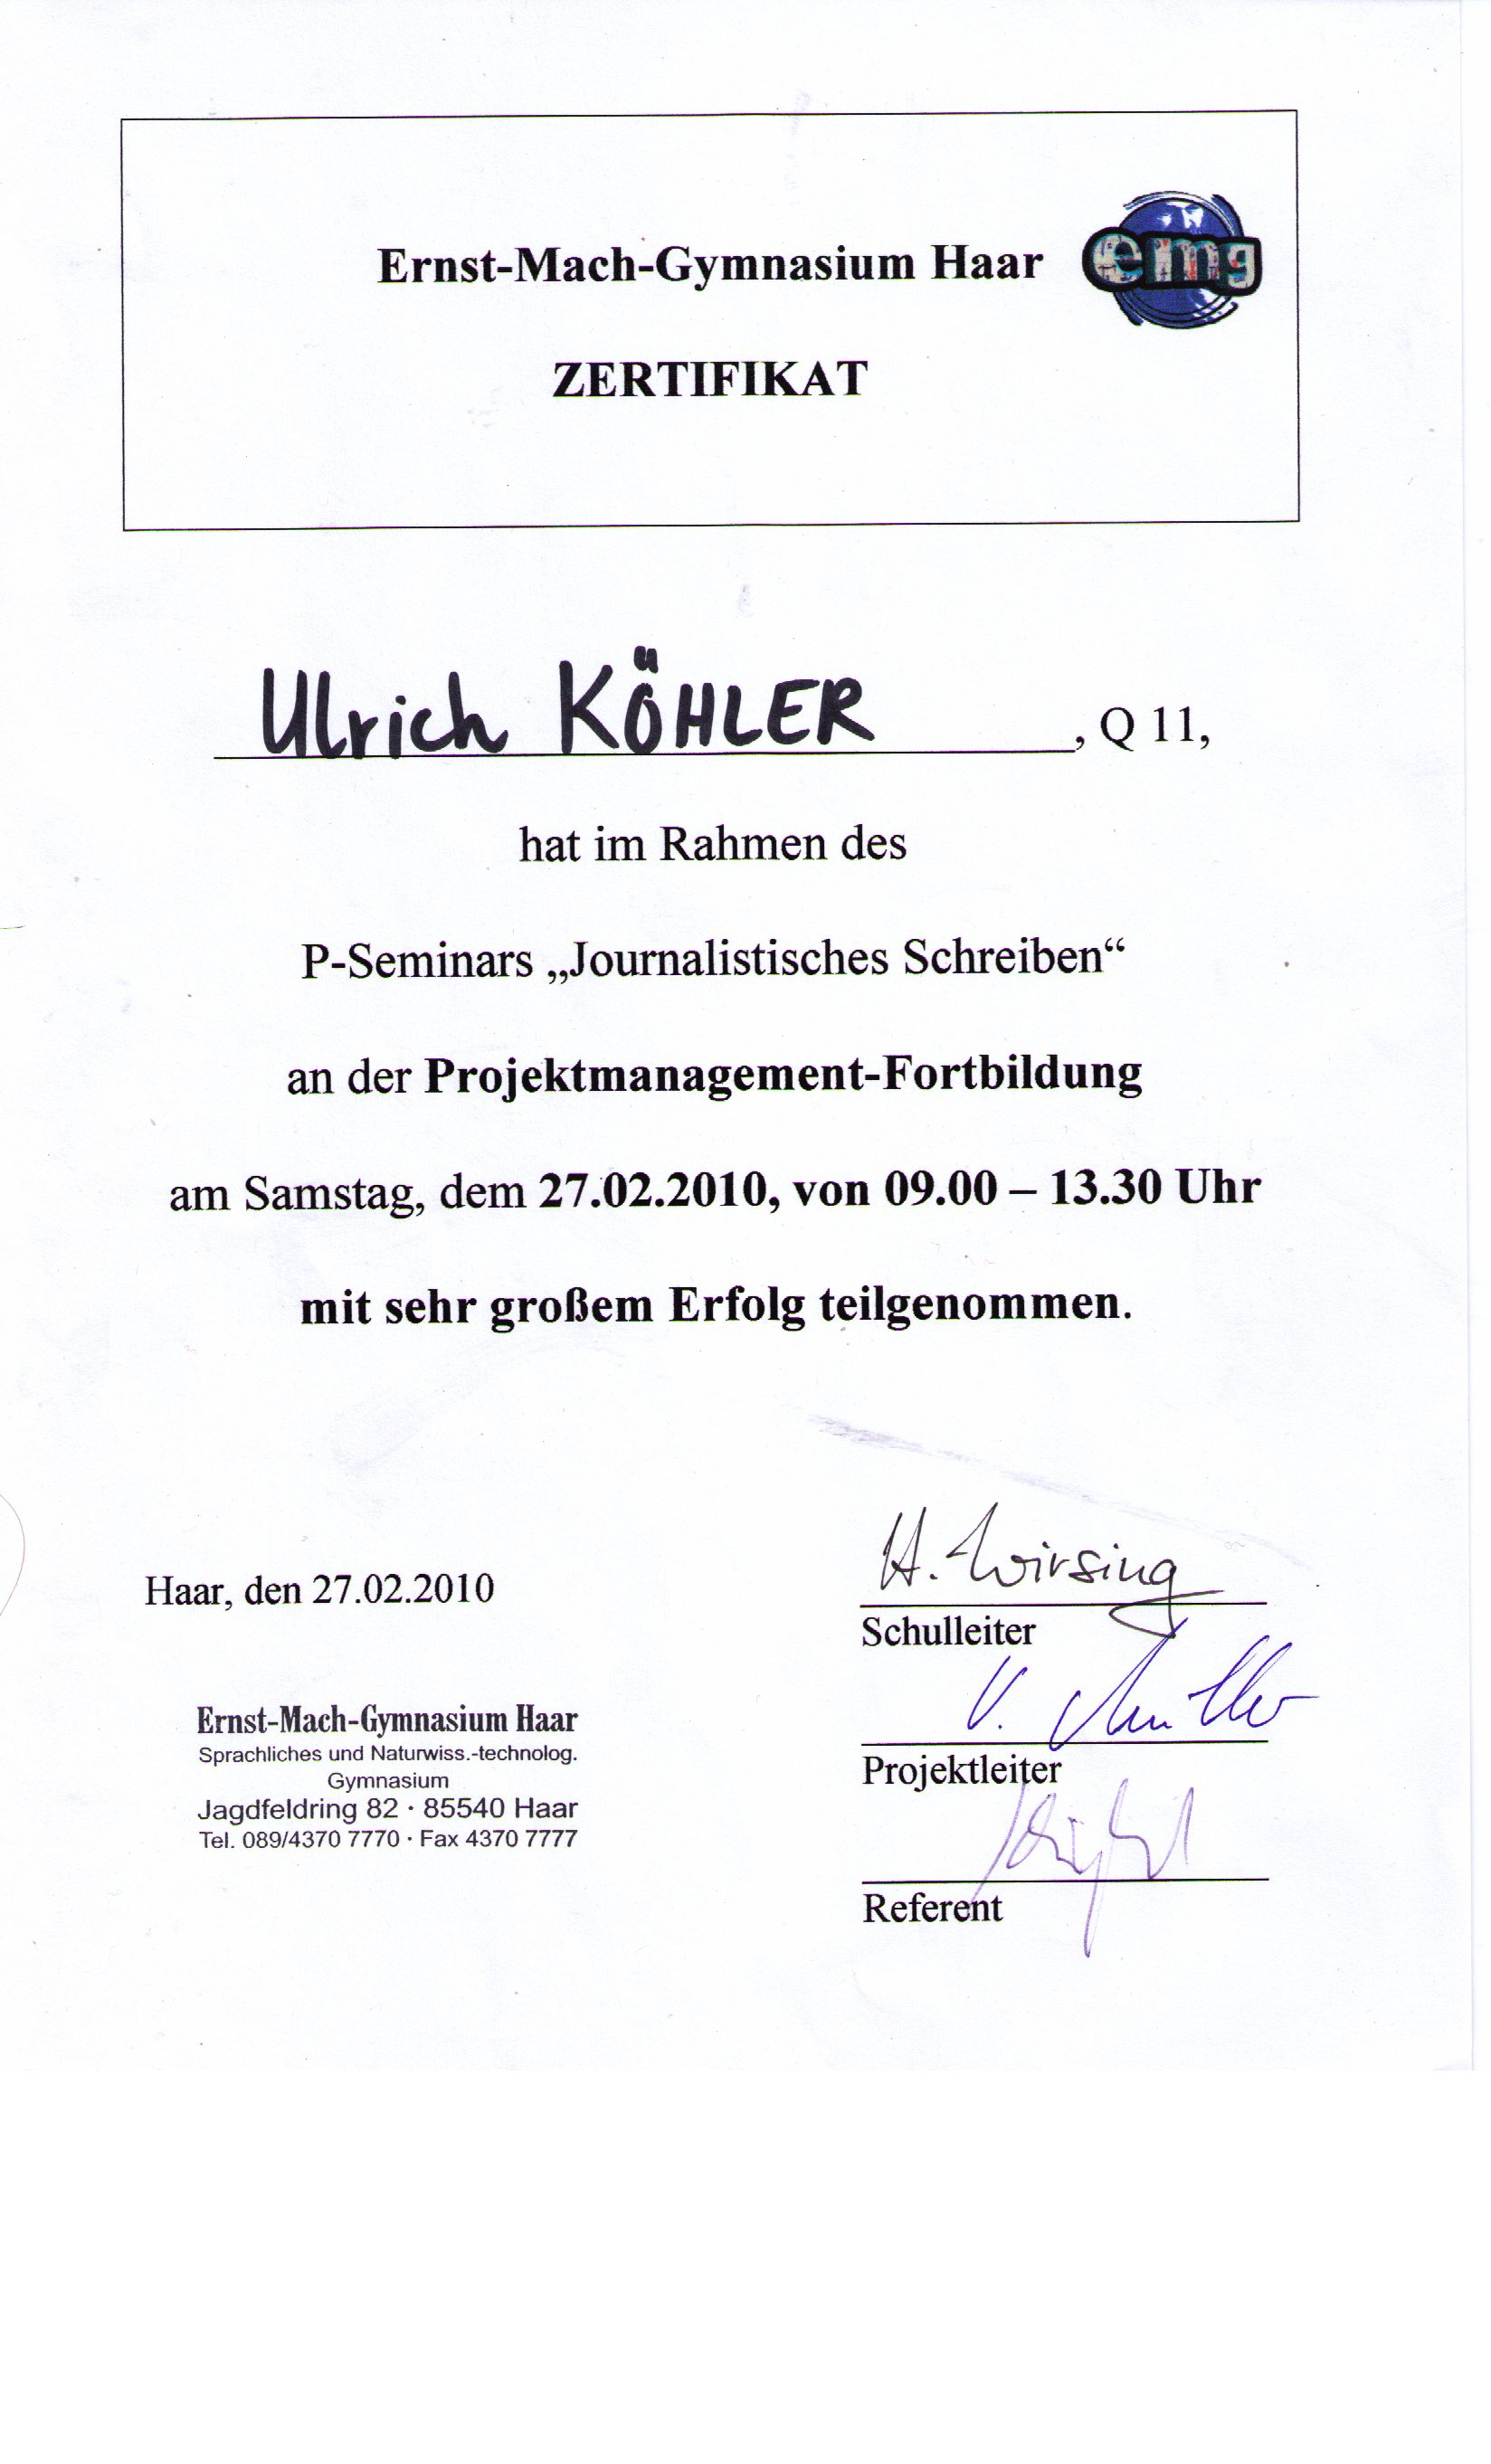
\includepdf{a1.jpg}

\includepdf{a2.pdf}
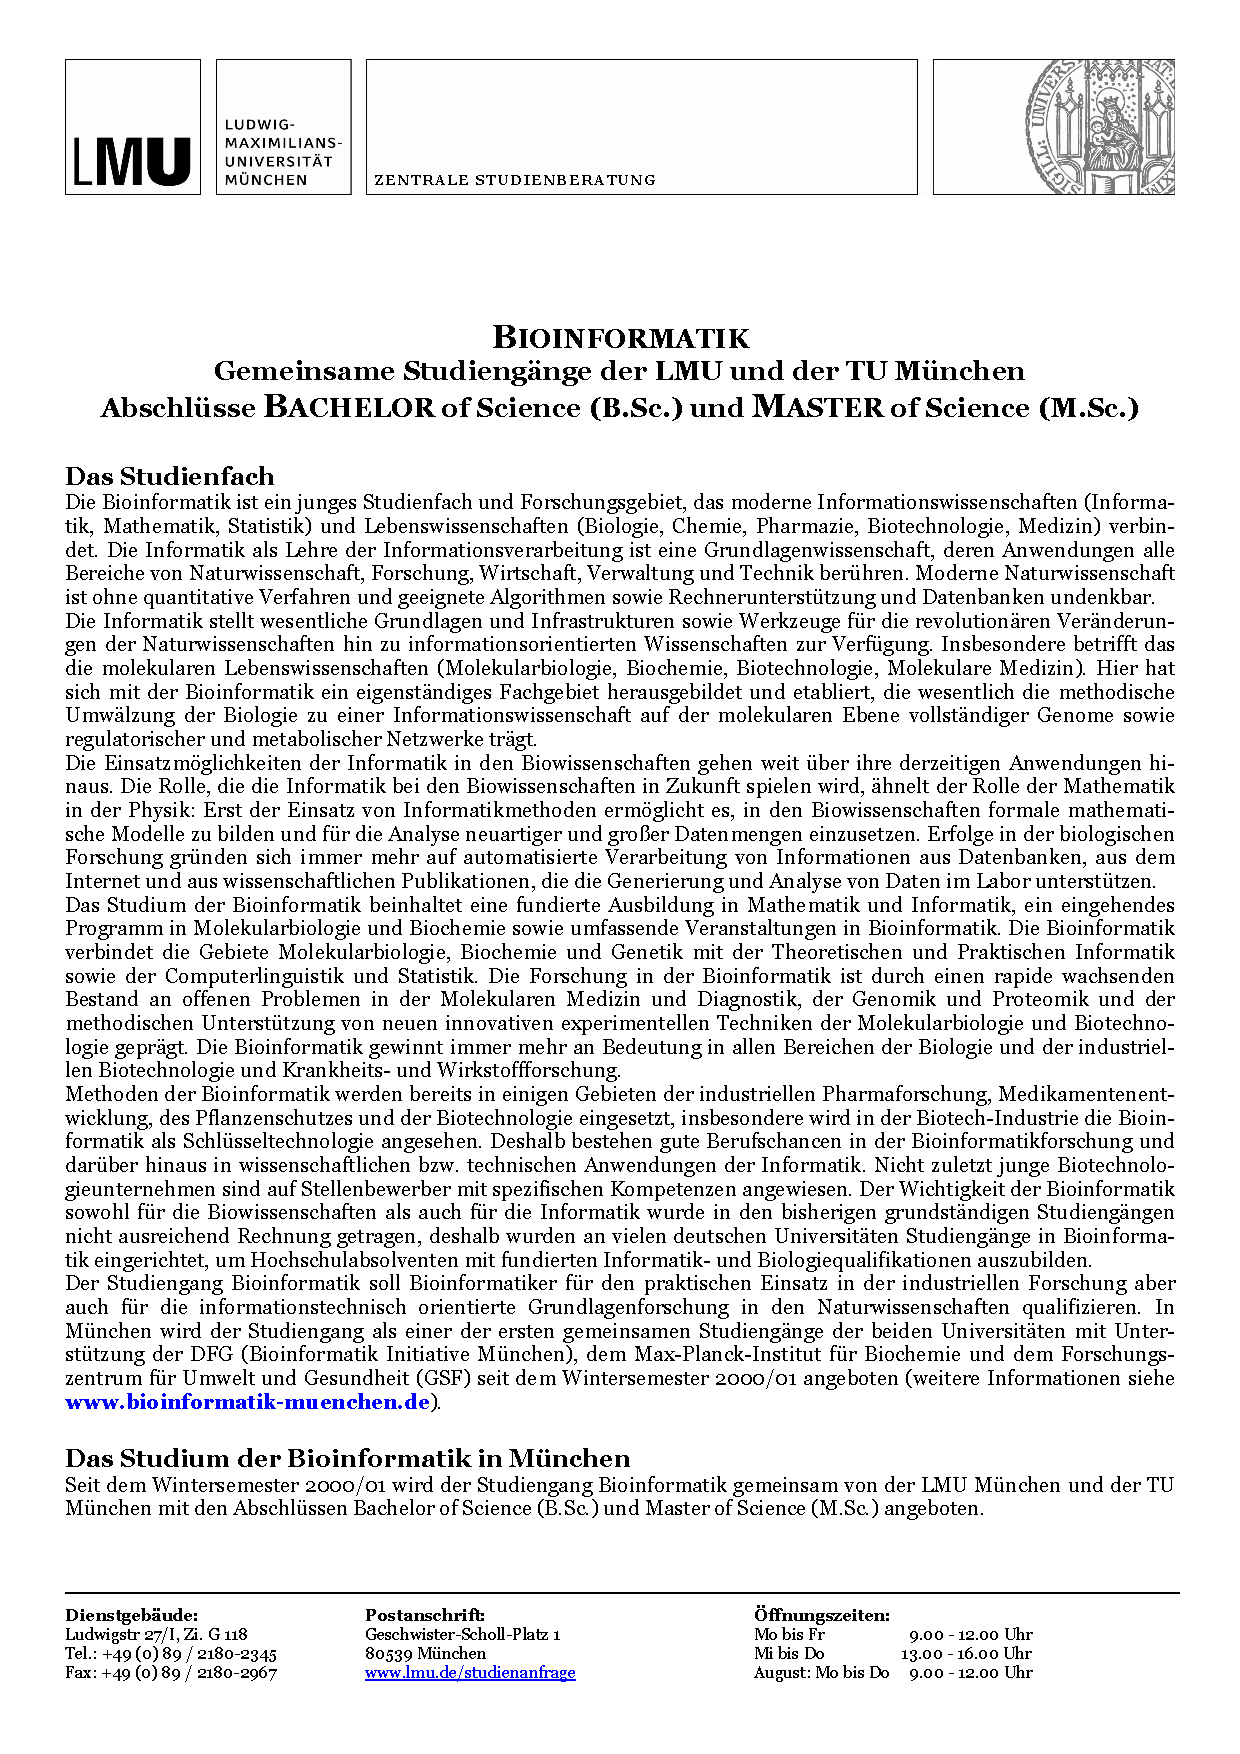
\includepdf{a3.pdf}

\includepdf{a4.pdf}
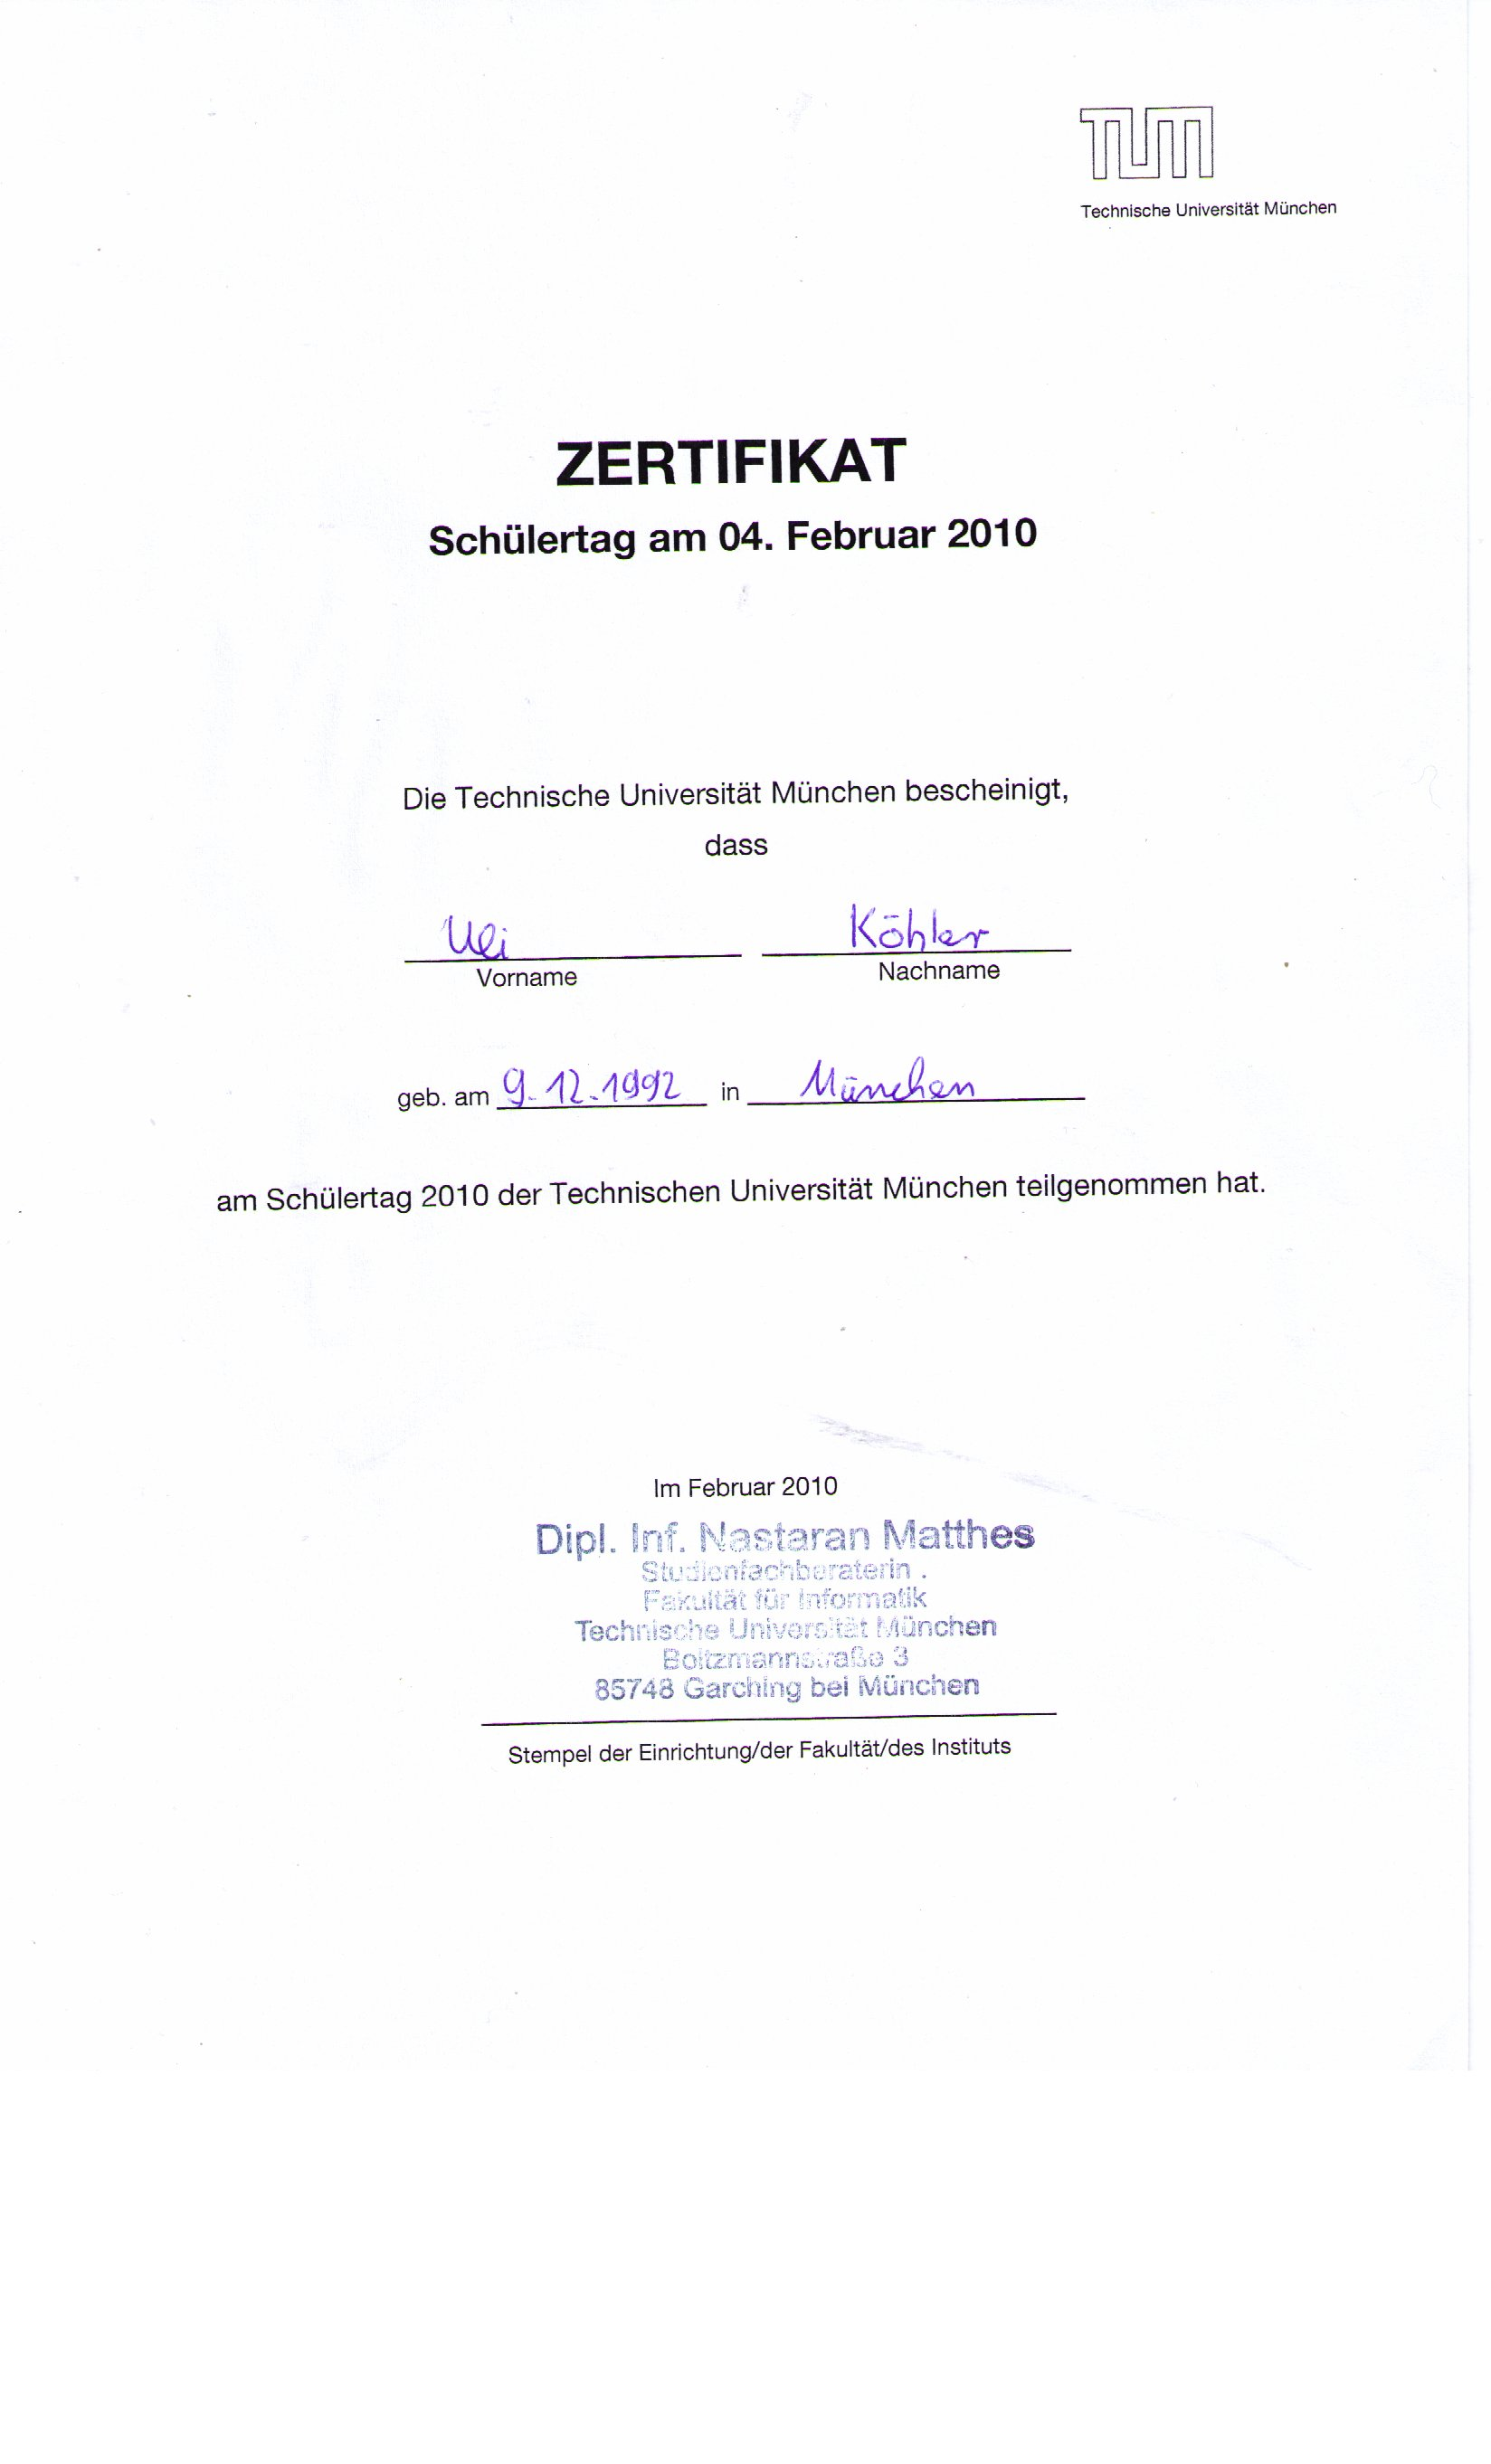
\includepdf{a5.jpg}
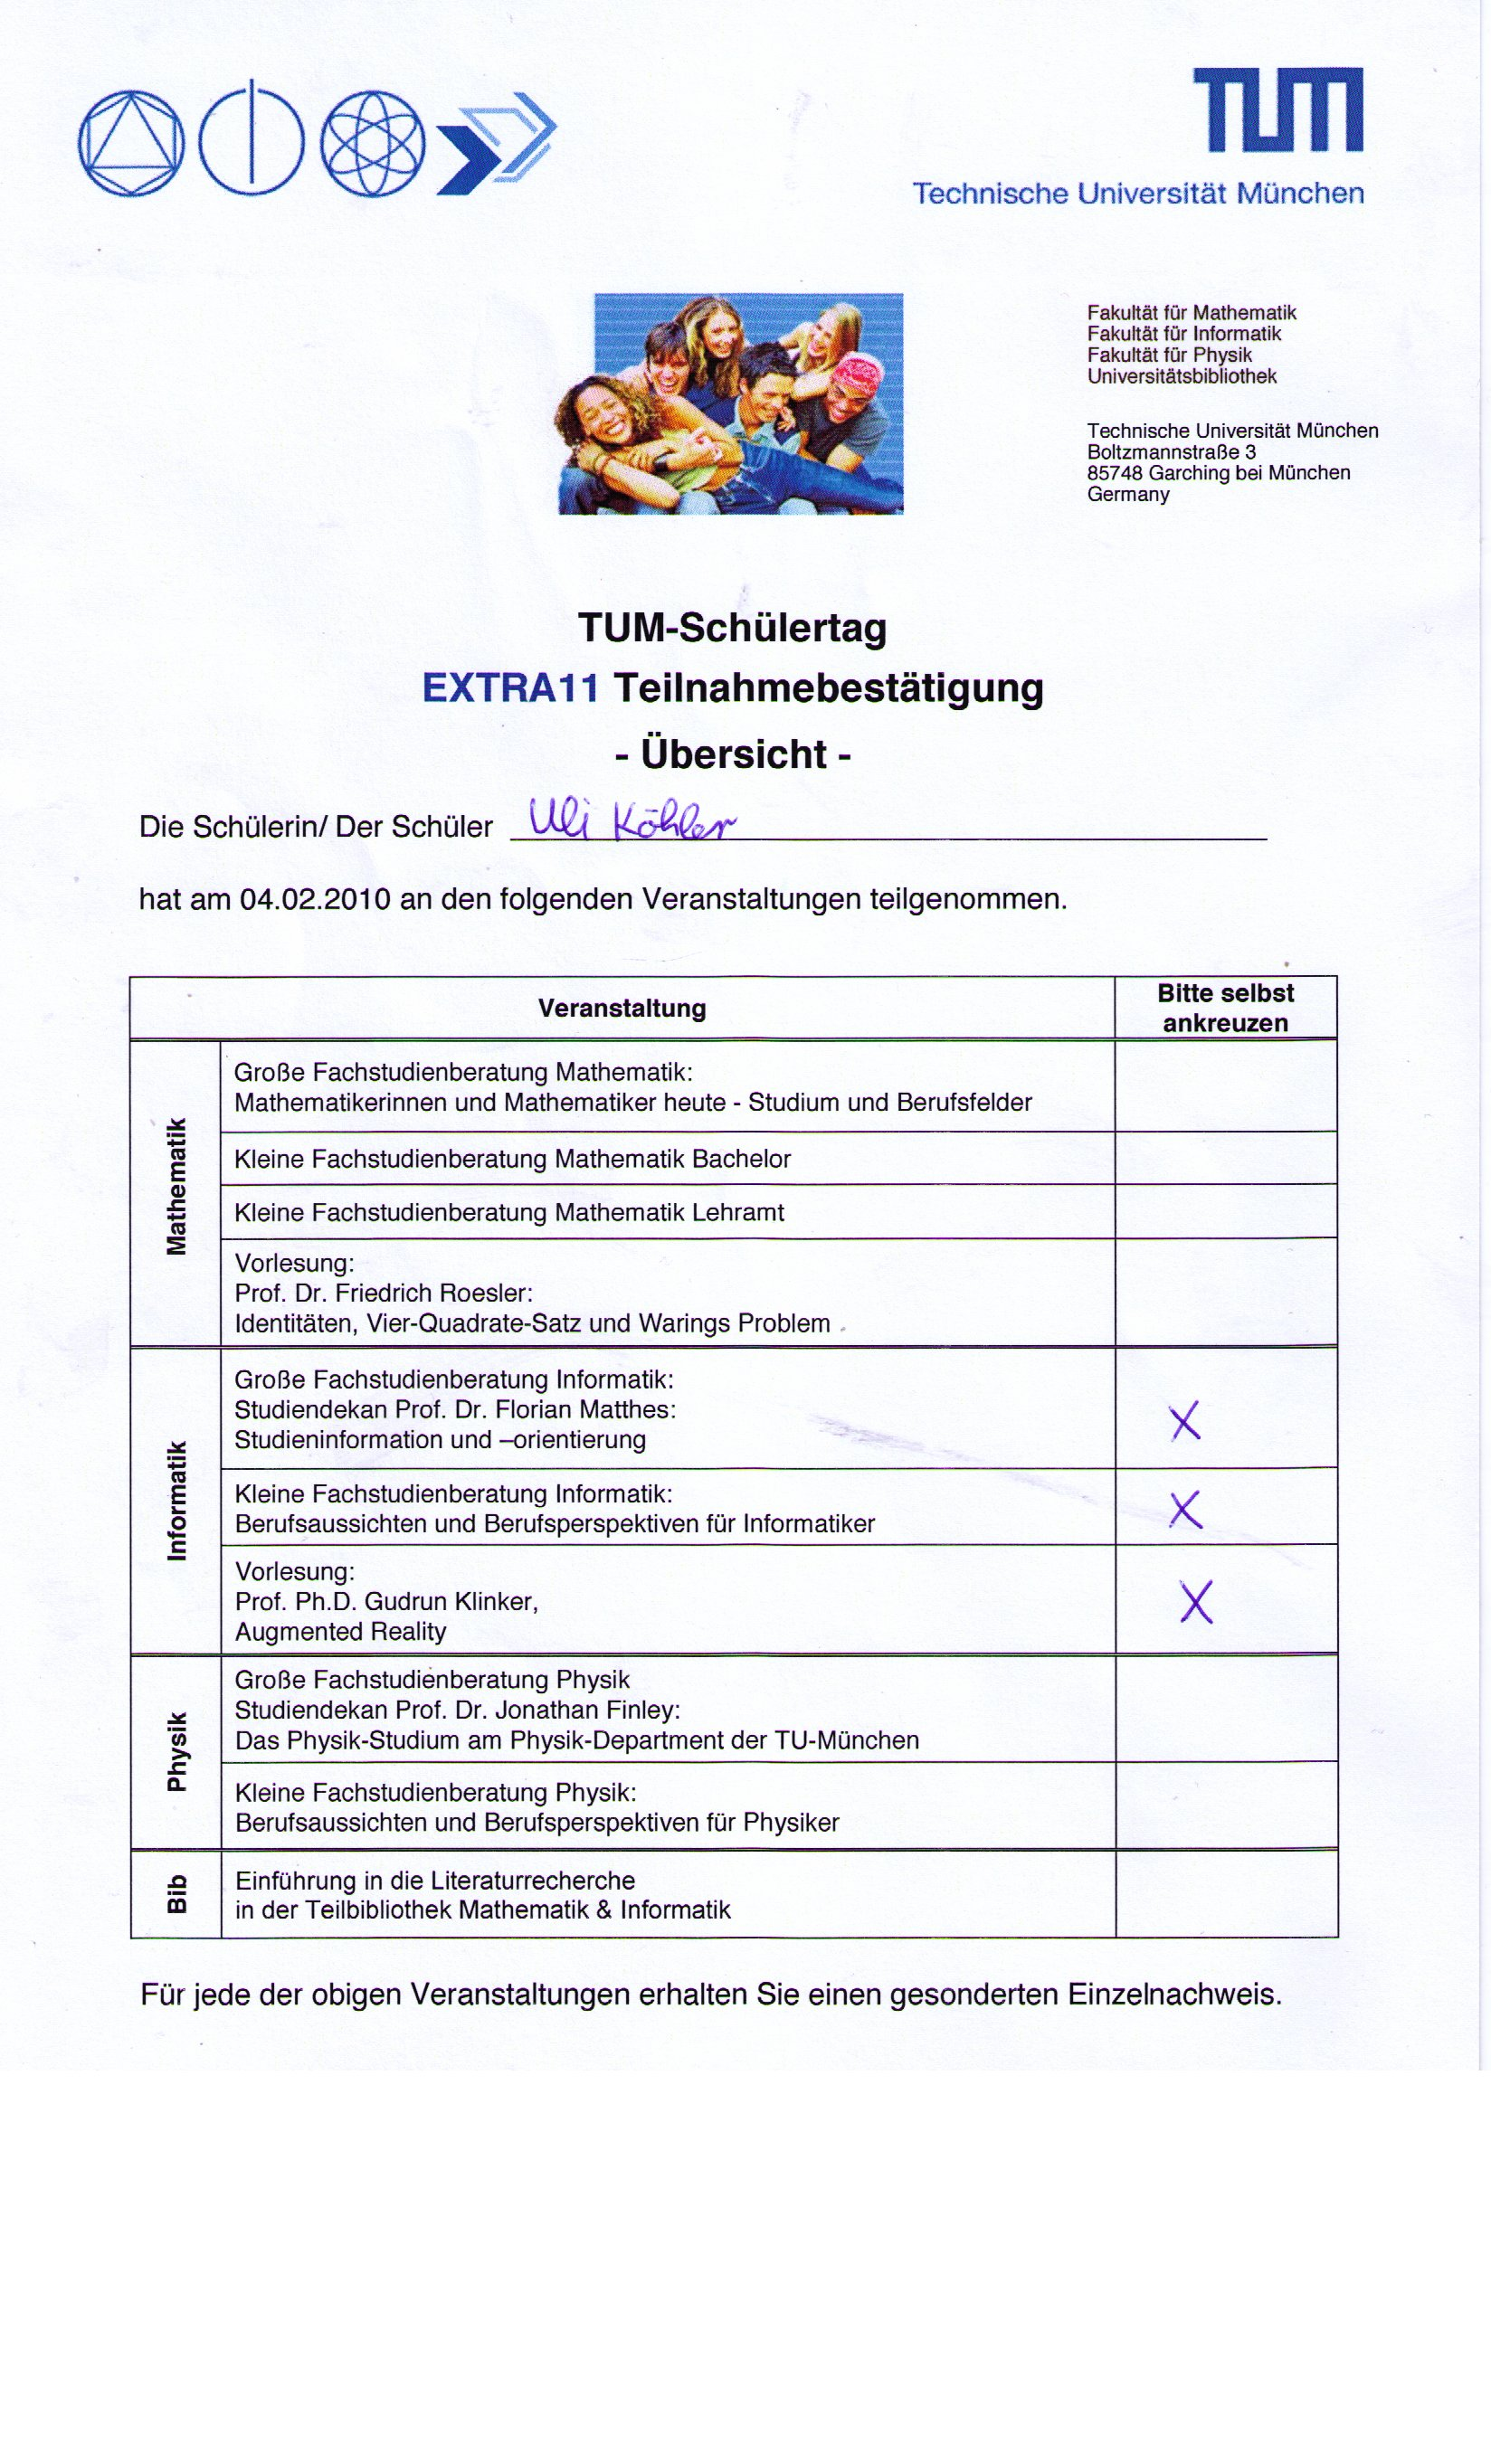
\includepdf{a6.jpg}
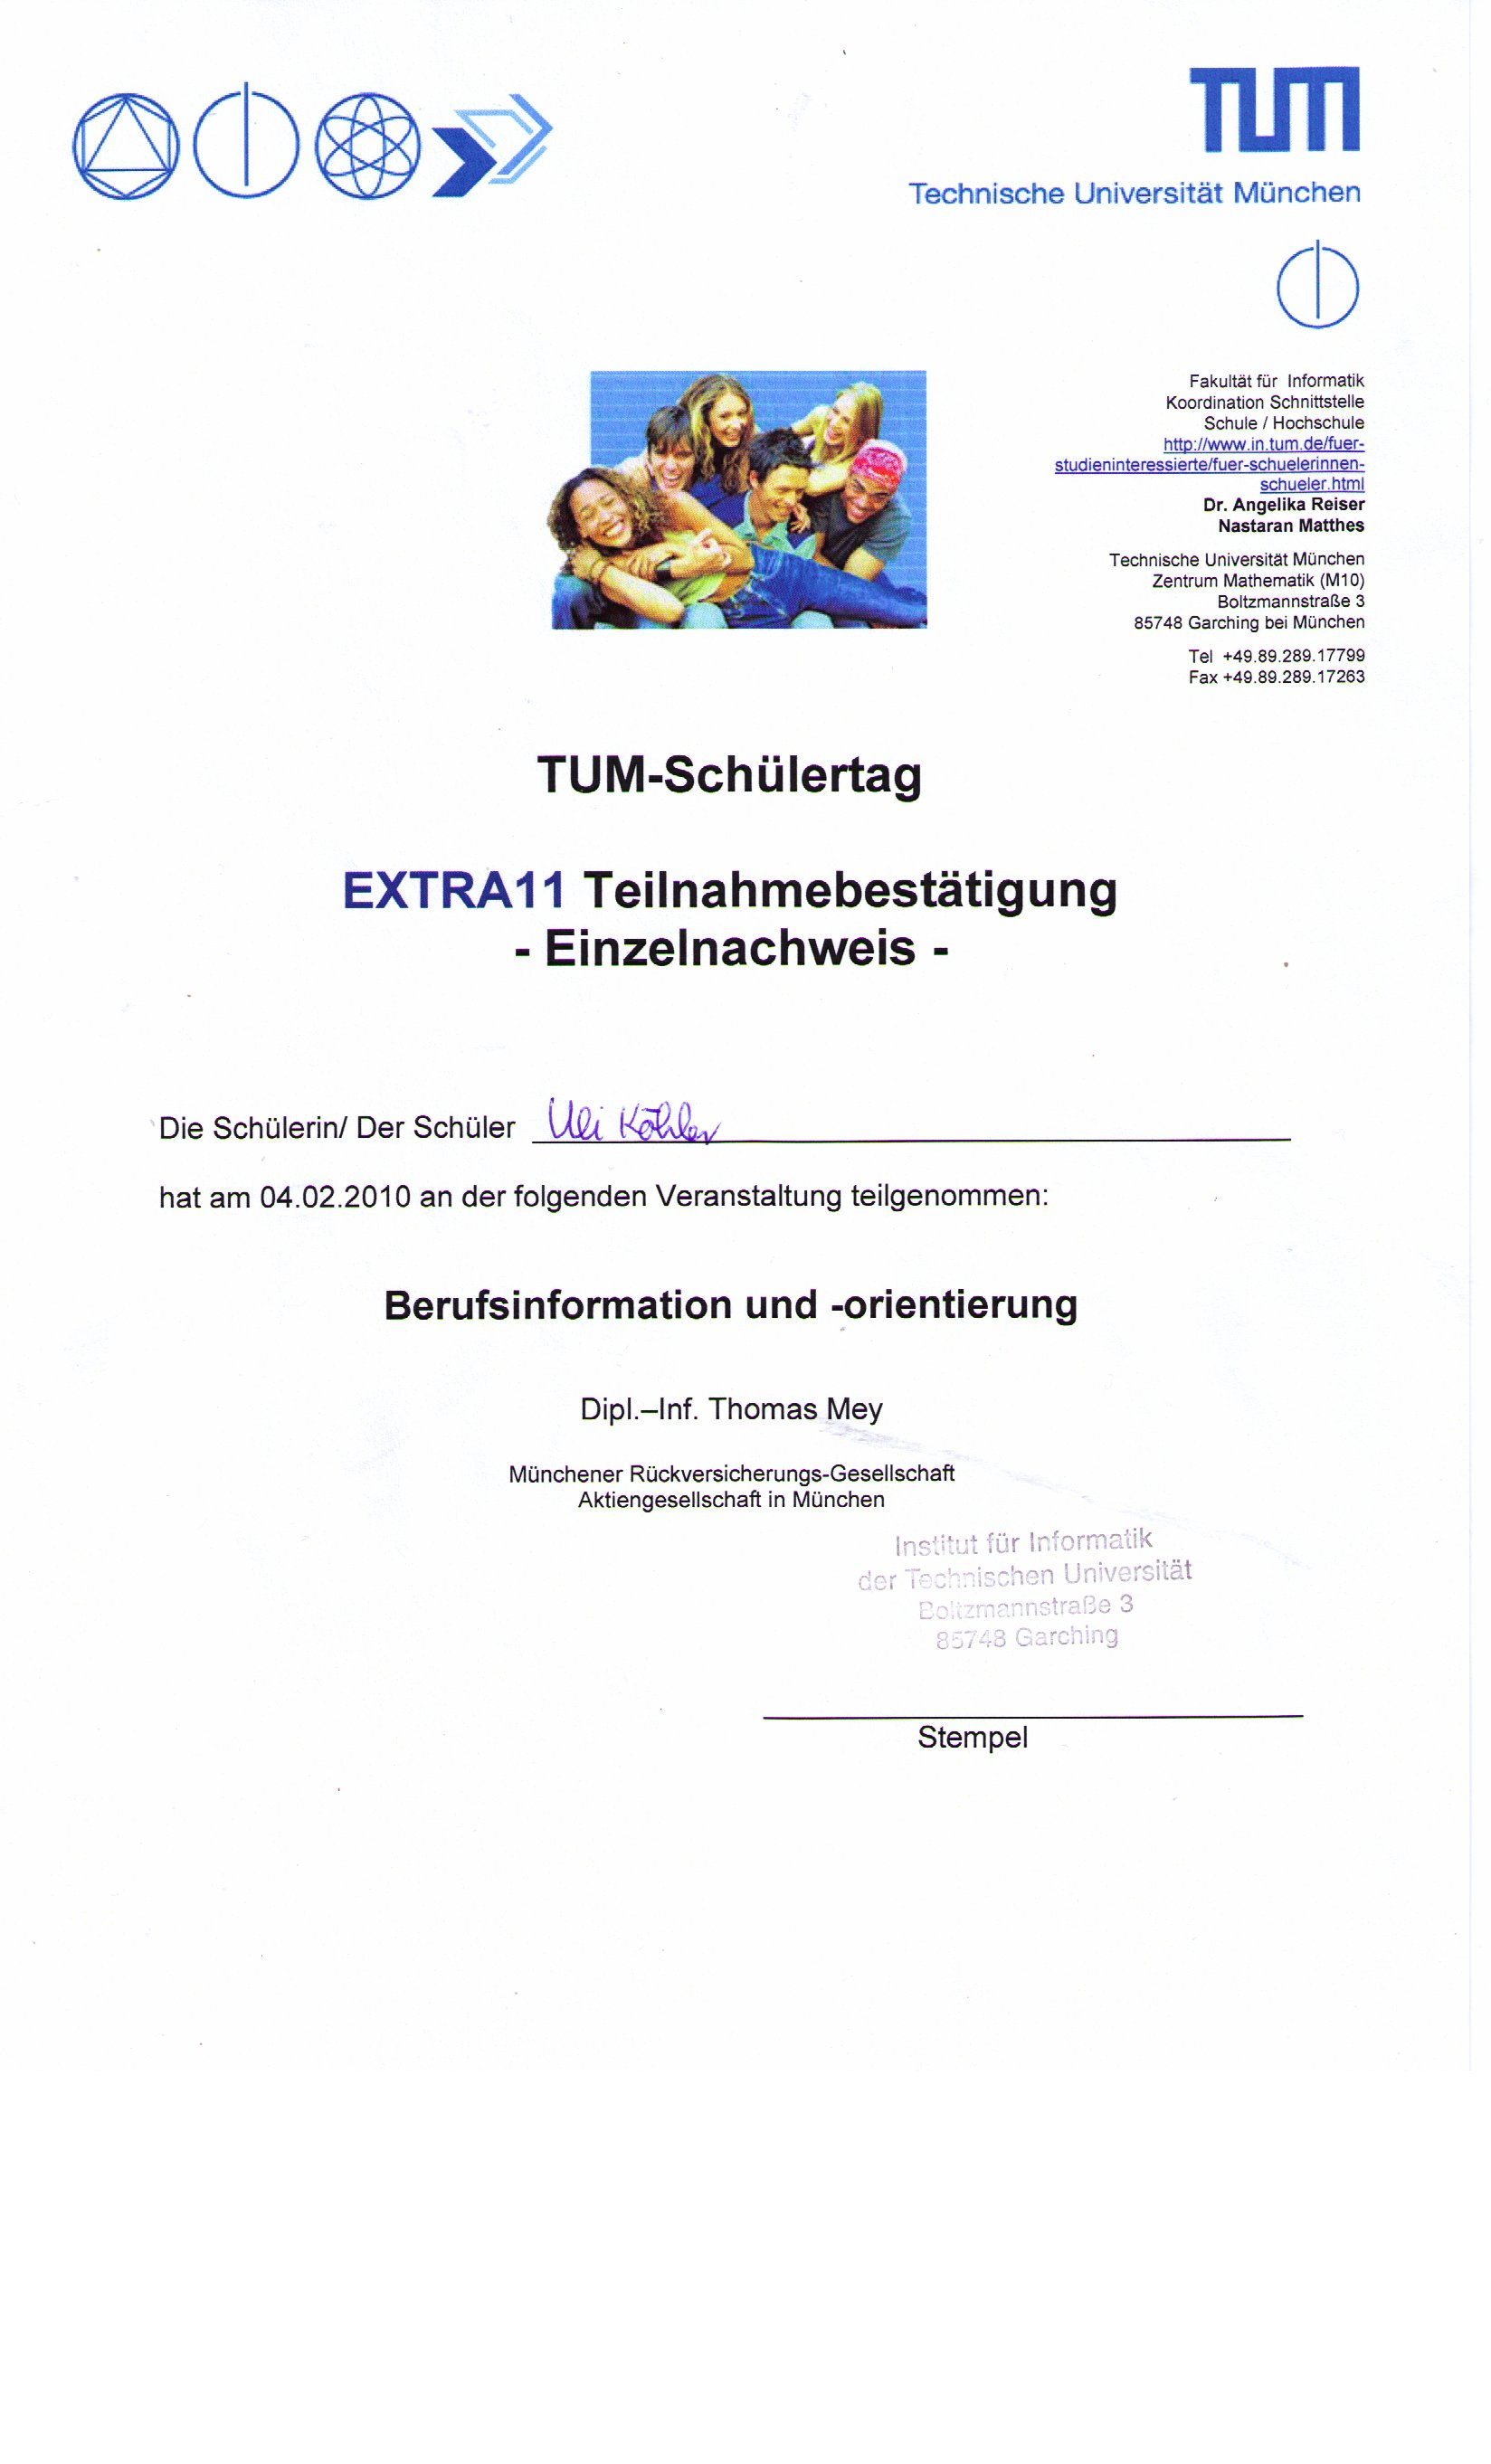
\includepdf{a7.jpg}
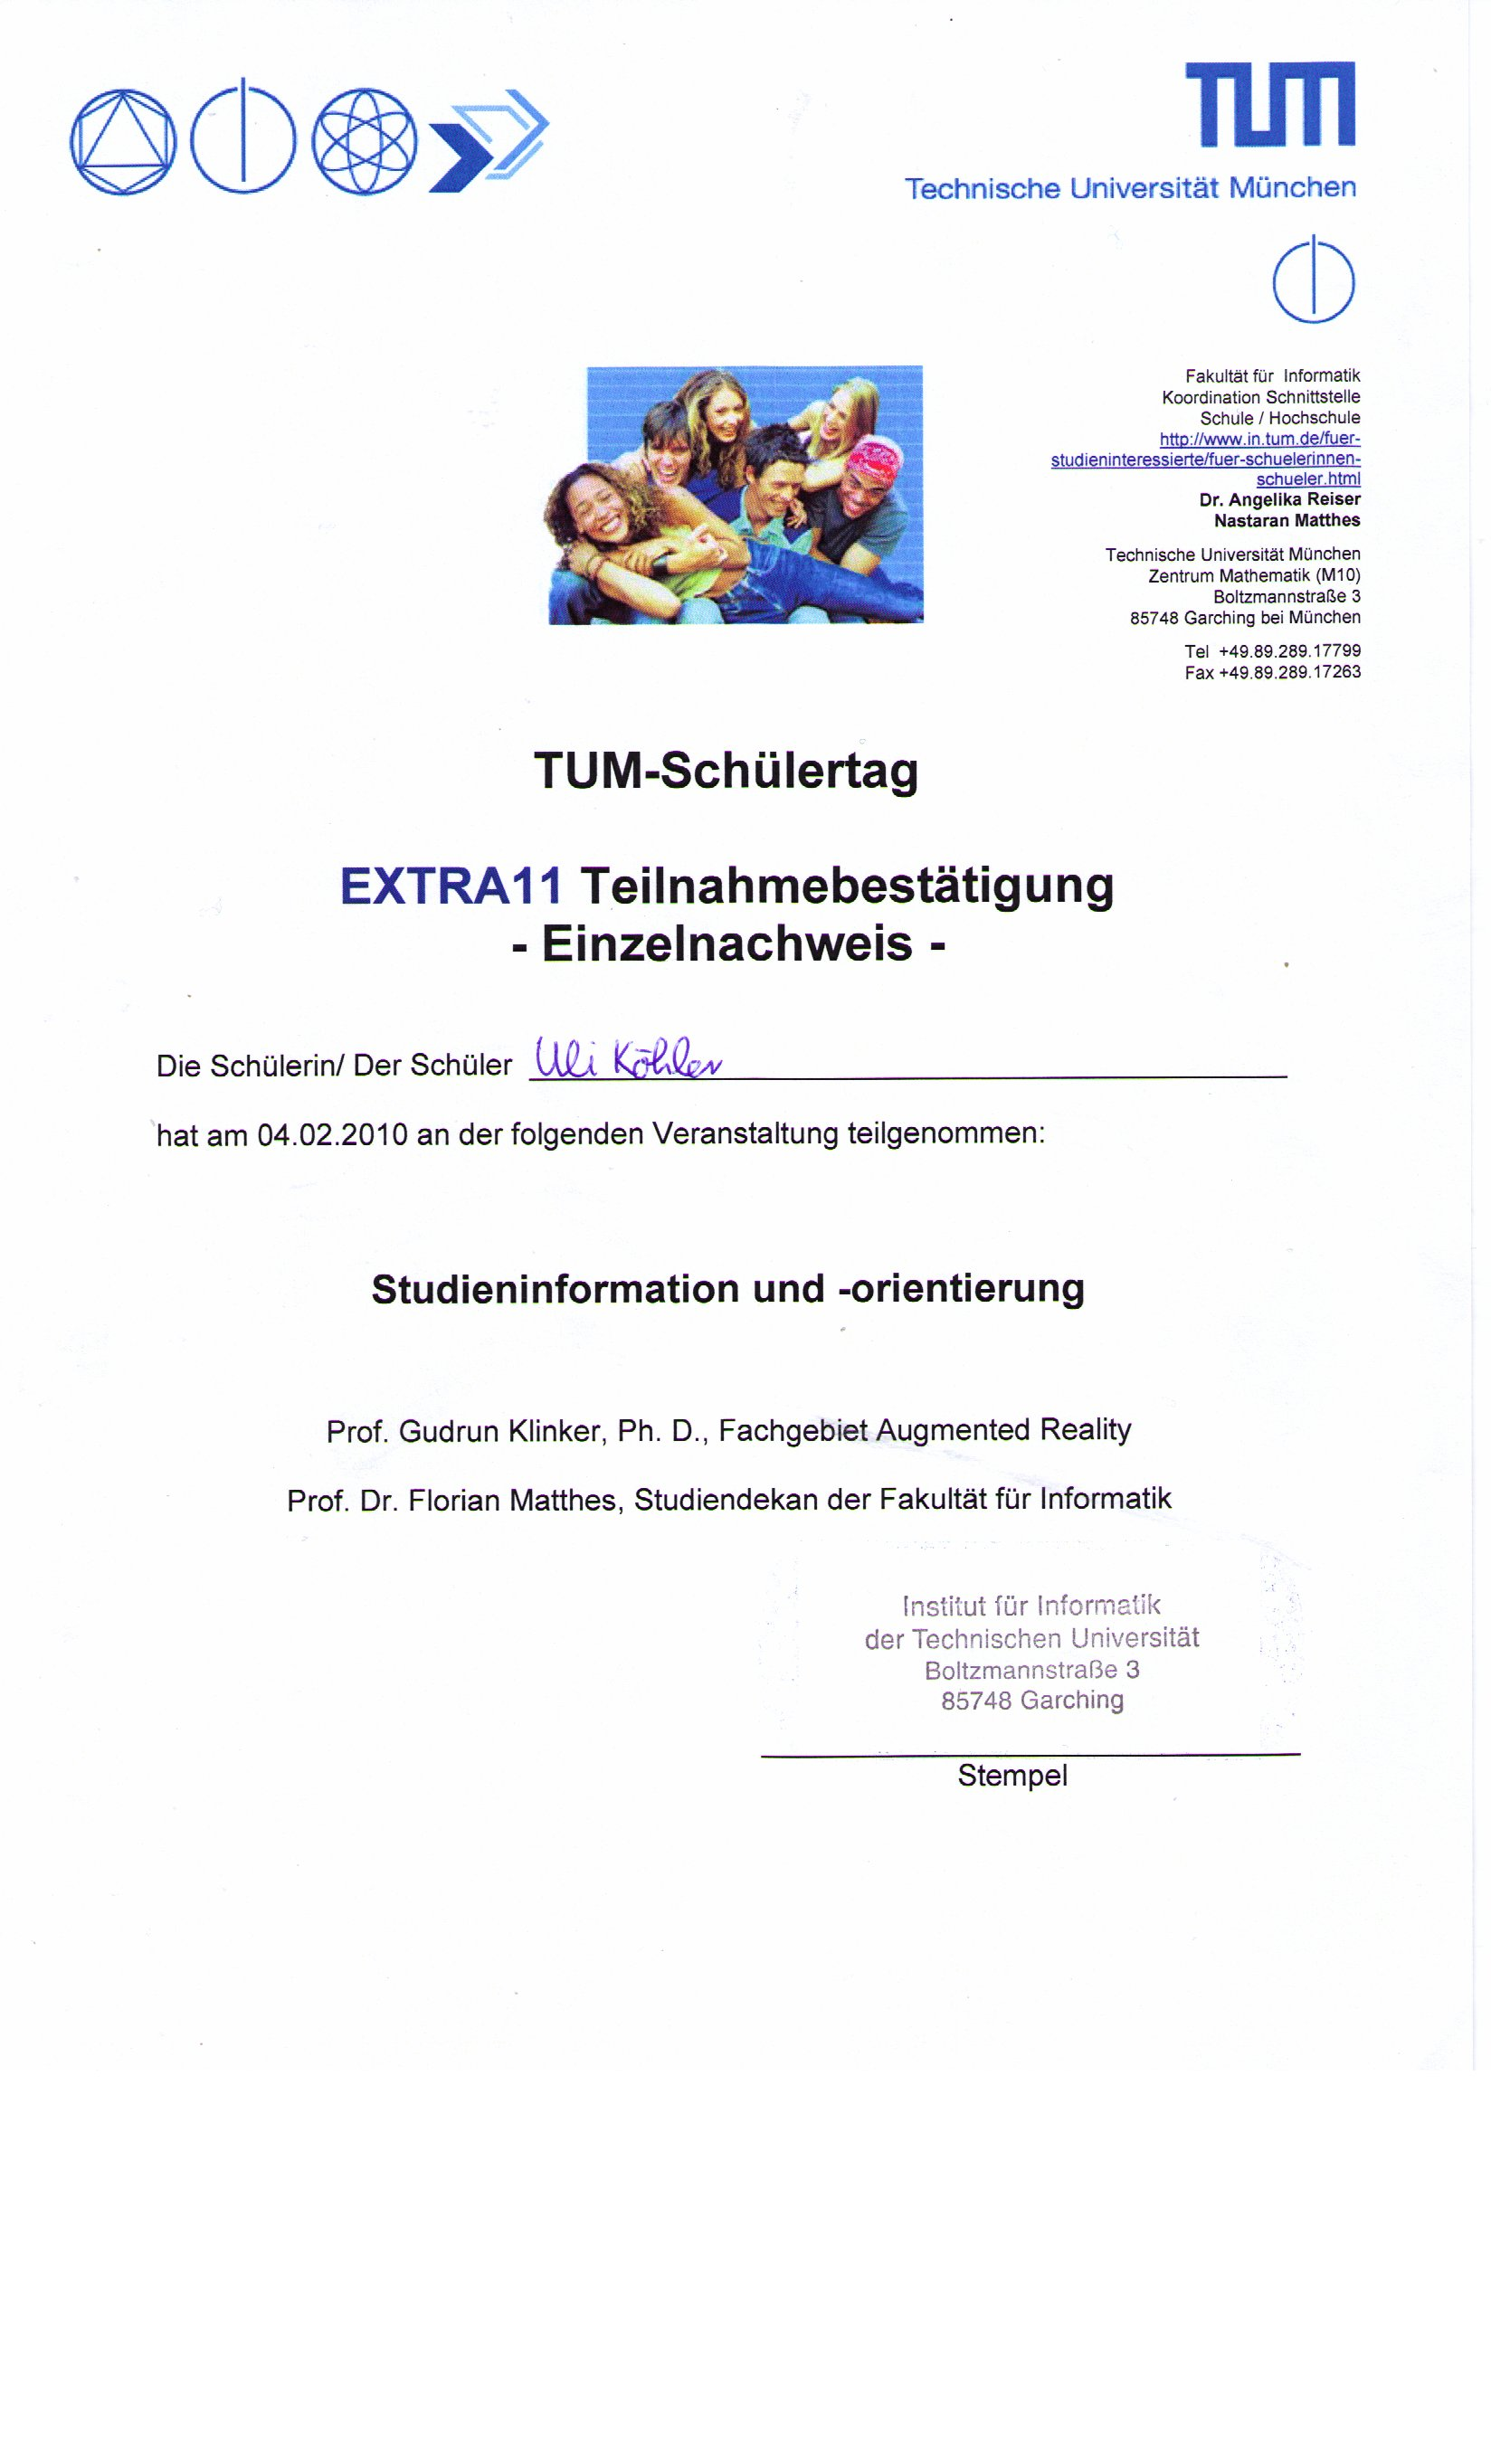
\includepdf{a8.jpg}
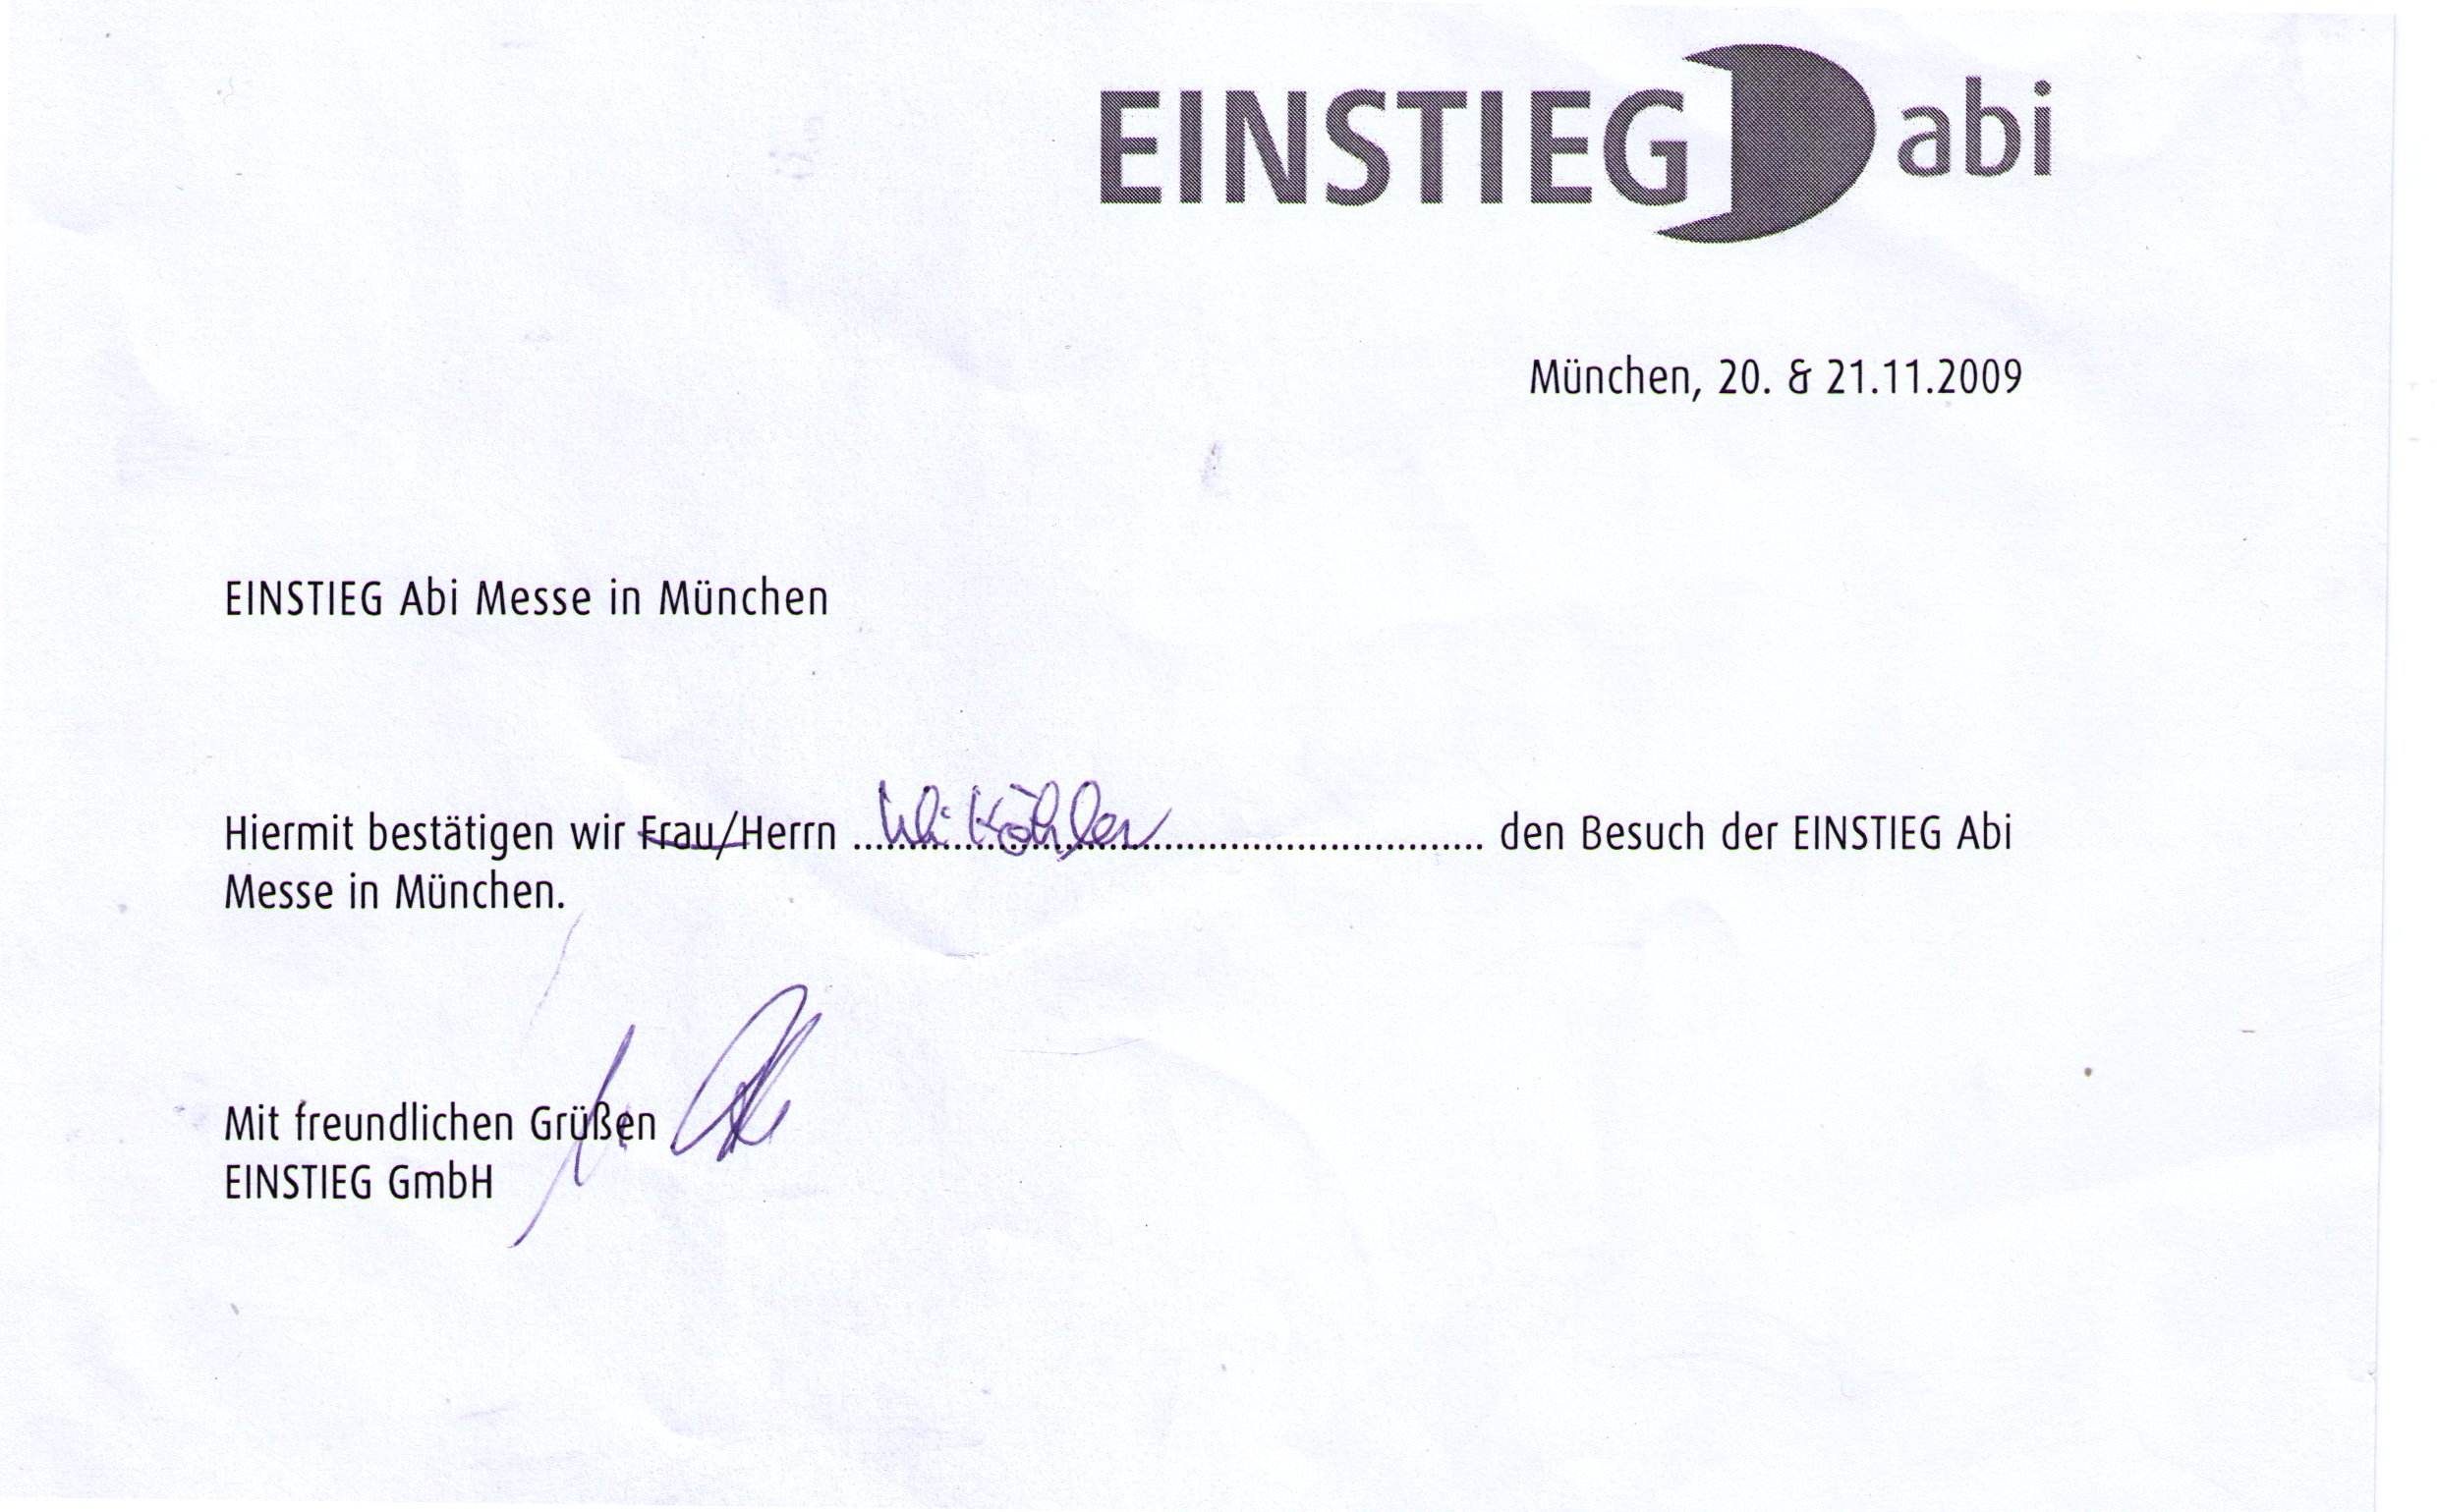
\includepdf{a9.jpg}
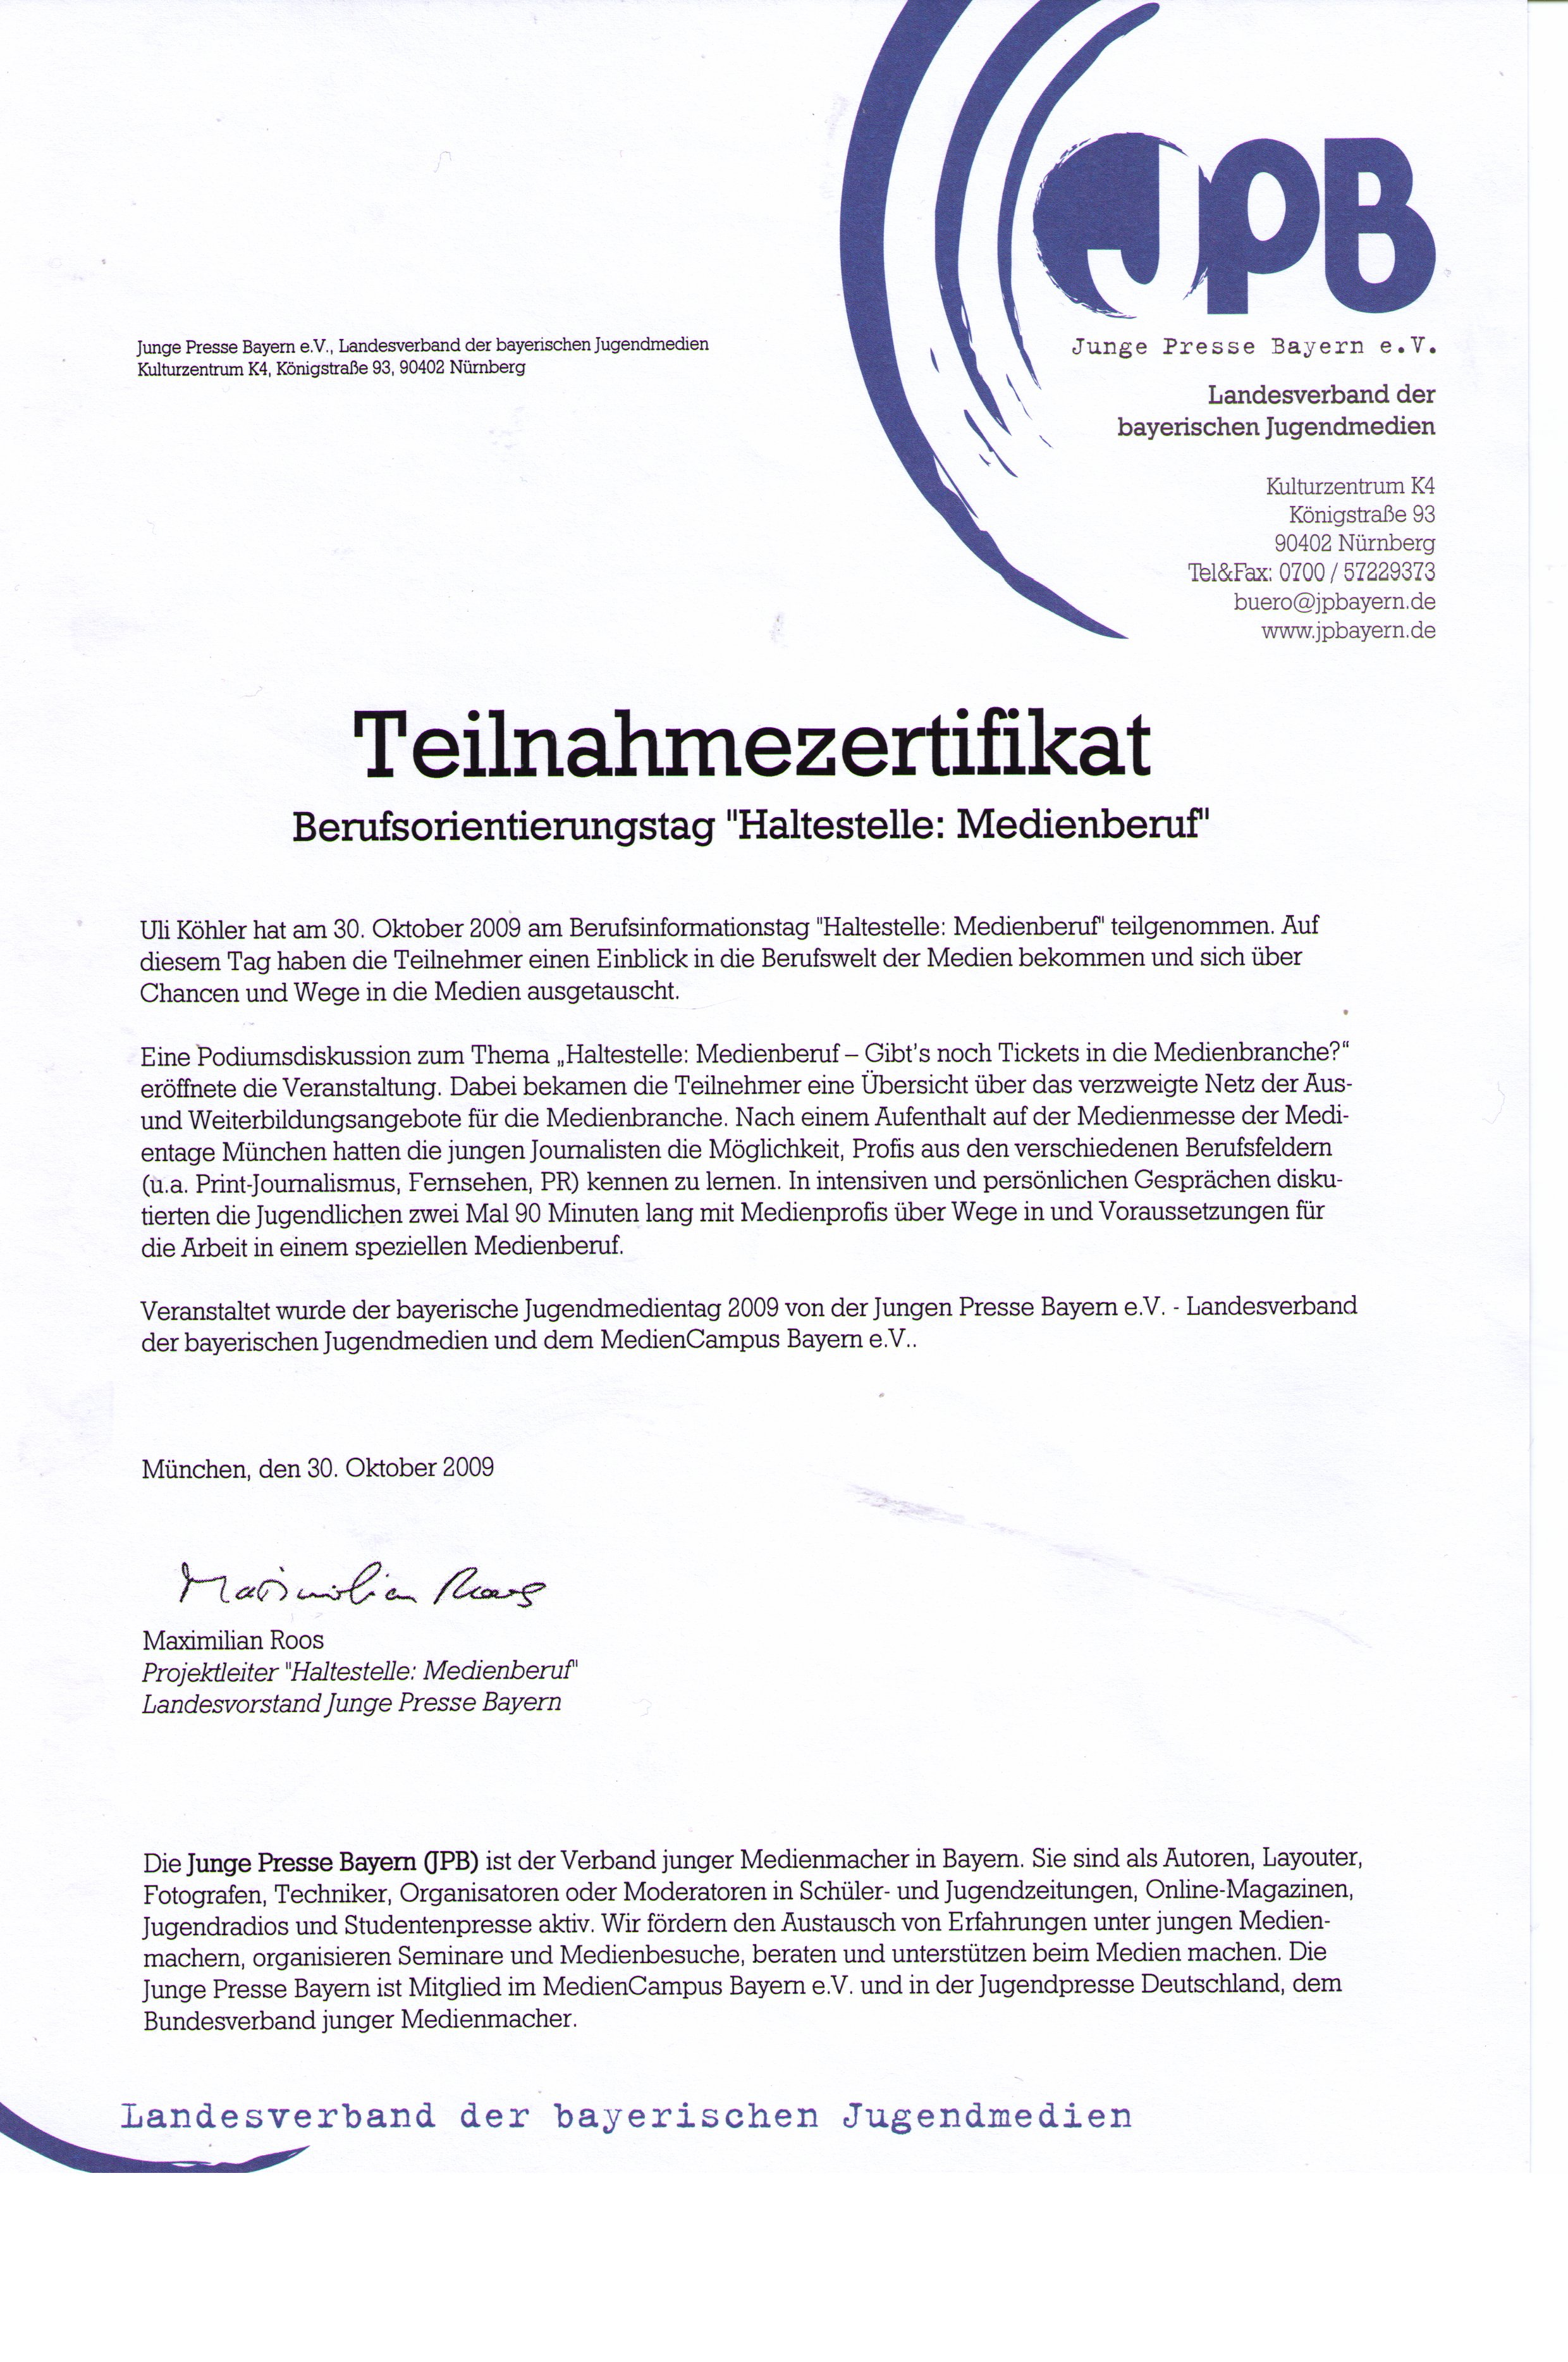
\includepdf{a10.jpg}
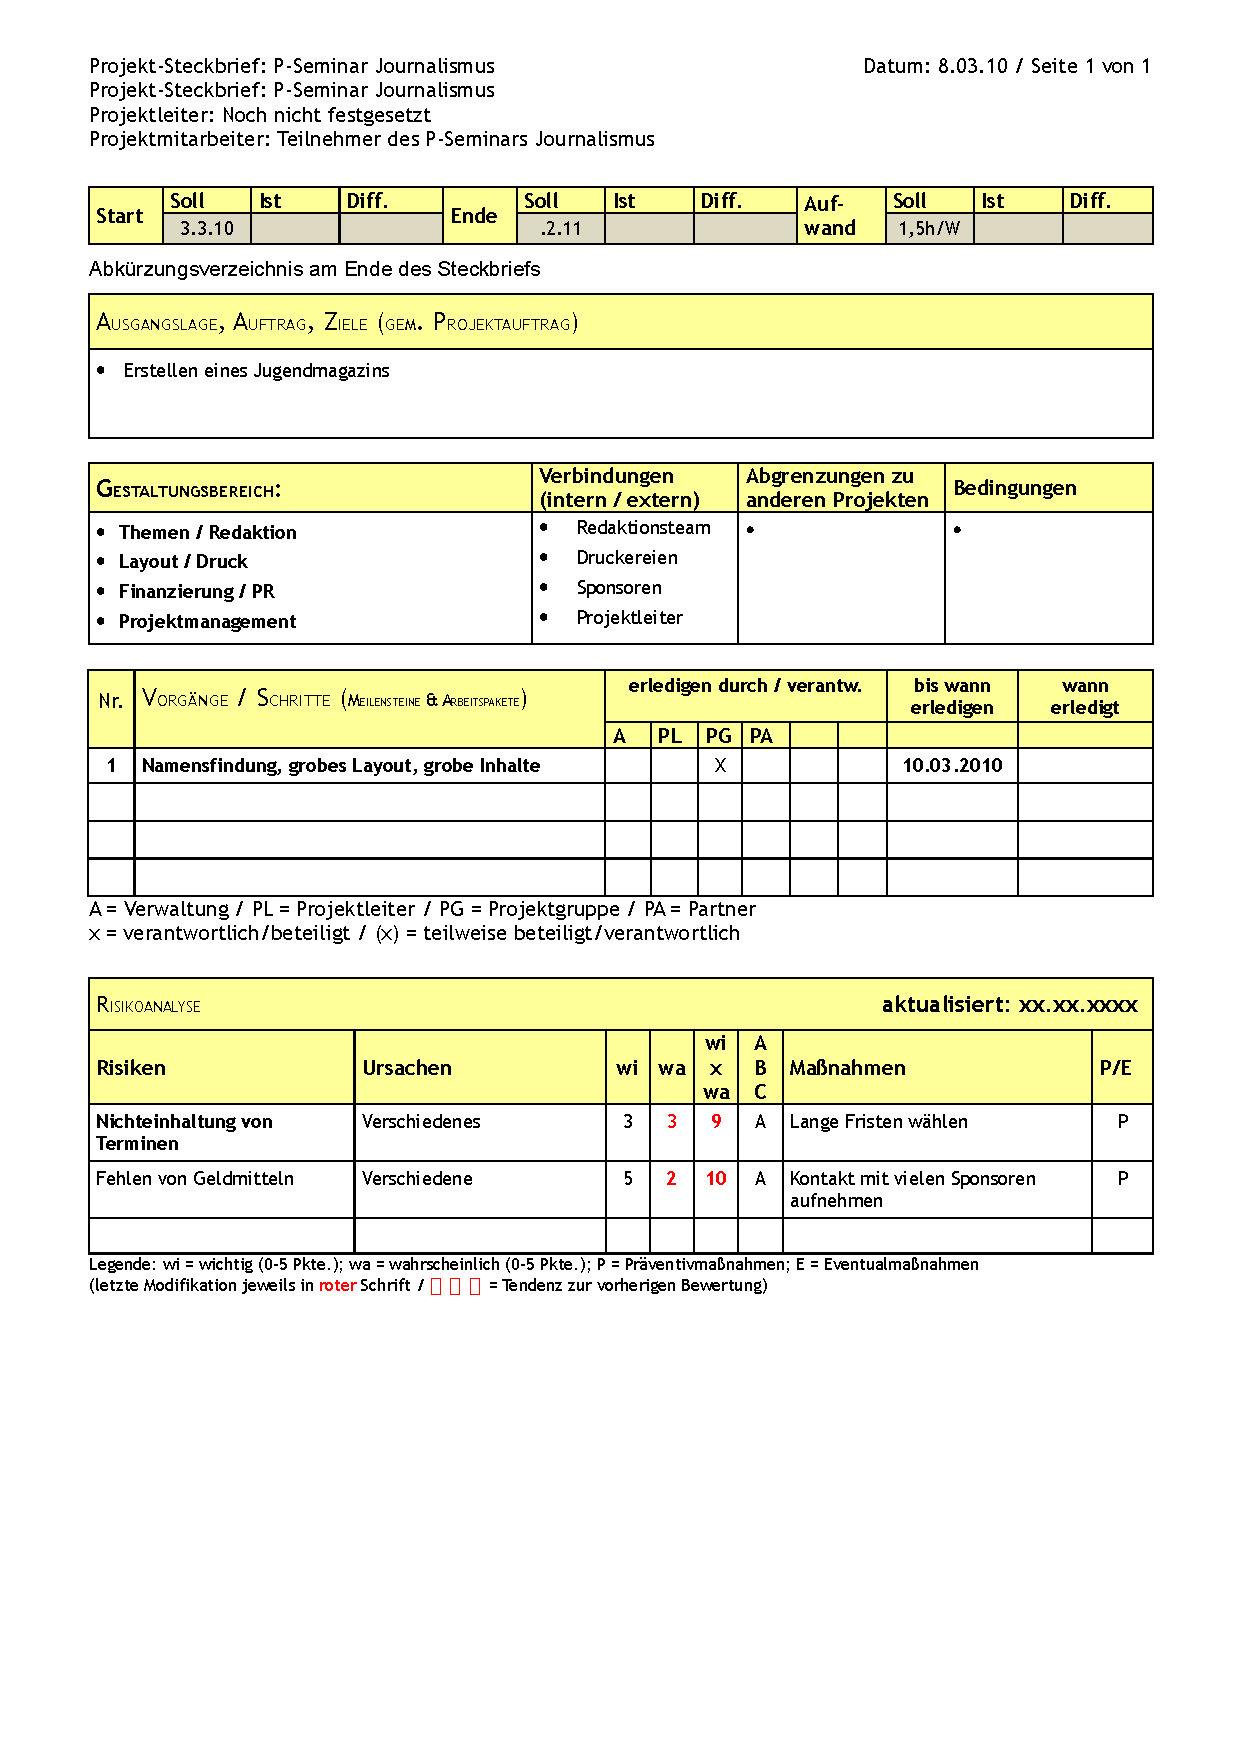
\includepdf{Steckbrief-Koehler.pdf}
\end{document}



